\section{Story Patterns (Christian und Marie)} \label{sec:StoryPatterns}

\todoch{Define concrete syntax for new elements. In particular, check syntax for links.}


\subsection{Story Pattern [CH]}
\label{sec:StoryPatterns:storyPattern}

Story Patterns are typed attributed graph transformation rules with inheritance (cf. Section \ref{sec:foundations:typedAttrGTS}) that may be embedded into an activity node of a story diagram (cf. Section \ref{sec:StoryDiagrams}). Type models for story diagrams can be created, e.g., by using EMF Ecore \cite{SBP+08}.  Using a type model enables use of inheritance and polymorphism for matching nodes.
This allows specifying graph replacement rules for object-oriented models.

\todoch{Should we provide an example for a type model here? Maybe we should have a section introducing type models (Ecore, UML, MOF) in the foundations.}

Story patterns are applied according to single pushout semantics using isomorphic matchings.
For enabling a concise notation of the graph transformation, story pattern apply a short-hand notation depicting the left-hand side (LHS) and the right-hand side (RHS) in a single, annotated graph. Nodes and edges being created (or deleted) are annotated with \create (or  \destroy, respectively).

Figure \ref{fig:simpleStoryPattern} shows an example of a single story pattern that creates a new method declaration in an interface and delegates the target of a call to this new method.

\begin{figure}[htbp]
  \centering
  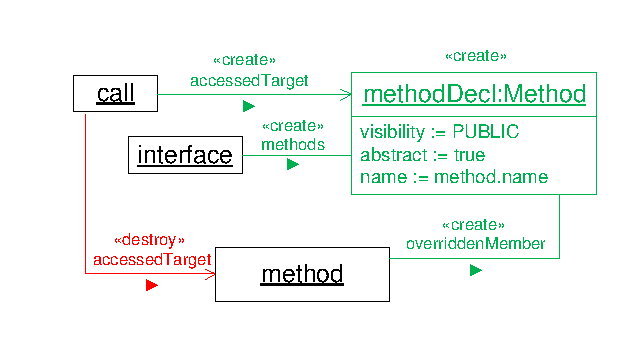
\includegraphics[scale=1.0]{figures/SimpleStoryPattern}
  \caption{Simple Story Pattern}
  \label{fig:simpleStoryPattern}
\end{figure}

In the example, the nodes \fe{call}, \fe{interface}, and \fe{method} are bound objects (cf. Section \ref{sec:StoryPatterns:binding:states}), i.e., they are already matched. When applying the story pattern, the link from \fe{call} to \fe{method} will be deleted. Thereafter, the node \fe{methodDecl} of type \fe{Method} will be created along with the three links pointing to it. Upon creation, the attributes \fe{visibility}, \fe{abstract}, and \fe{name} are initialized with the specified values.

In a story pattern, we call all nodes and links that do not carry an annotation the \emph{core graph} of the story pattern. Then, the LHS of the story pattern consists of the core graph and all nodes and links annotated with \destroy. Accordingly, the RHS of the story pattern consists of the core graph and all node and links annotated with \create.

\subsection{Objects and Object Variables [MCP]}
\label{sec:StoryPatterns:objects}

\todomcp{each connected component must contain at least one bound object
variable}

%Object variables represent the objects defined in a story pattern.
%They are identified by their name.
%The objects are instances of classes of the underlying classmodel (cp. Section \ref{typedGraphTransformations}).
%Thus, the object variables are typed by classes from this model.

%\begin{figure}[htbp]
%\begin{center}
%  \includegraphics[width=0.25\textwidth]{figures/objectVariable}
%  \caption{An object variable}
%  \label{fig:objectVariable}
%\end{center}
%\end{figure}
%Figure \ref{fig:objectVariable} shows an object variable with the name \texttt{methodDecl} and the type
%\texttt{Method}.

\todomcp{Primitive Variables are part of this section, too; concrete syntax like
object variables; binding expressions for initialization, see figure
\ref{fig:primitiveVariable}; primitive variables are typed over EDataType; they exist beyond the end of the Activity}

\begin{figure}[htbp]
  \centering
  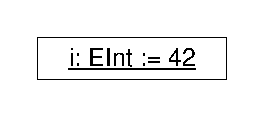
\includegraphics[scale=0.6]{figures/PrimitiveVariable}
  \caption{Primitive variable with value assignment}
  \label{fig:primitiveVariable}
\end{figure}

\todomcp{Links to primitive variables: special LinkVariable, typed over
EStructuralFeature}

\subsection{Links and Link Variables [MCP]}
\label{sec:StoryPatterns:links}

\subsection{Binding of Variables [MCP]}
\label{sec:StoryPatterns:binding}

%Object variables and link variables have binding operators, binding states, and binding semantics.

\subsubsection{Binding Operators}
\label{sec:StoryPatterns:binding:operators}
%The binding operators define whether an element is to be created, deleted, or just matched.
%After all elements that are defined to be deleted or just matched have been matched, the model ist modified by creating
%and deleting the elements as defined. 

%Elements to be created are marked with the
%label \texttt{CREATE} and elements to be deleted are marked with the label \texttt{DESTROY}.

\subsubsection{Binding States}
\label{sec:StoryPatterns:binding:states}

\subsubsection{Binding Semantics}
\label{sec:StoryPatterns:binding:semantics}

\todomcp{Negative objects, Figure \ref{fig:negativeObjects}:
a) allowed; same semantics for the same situation with link not negative
b) not allowed because graph is not connected
c) allowed
d) allowed because a and b are both bound
e) not allowed
f) allowed; same semantics for the same situation with links not negative
}

\begin{figure}[htbp]
  \centering
  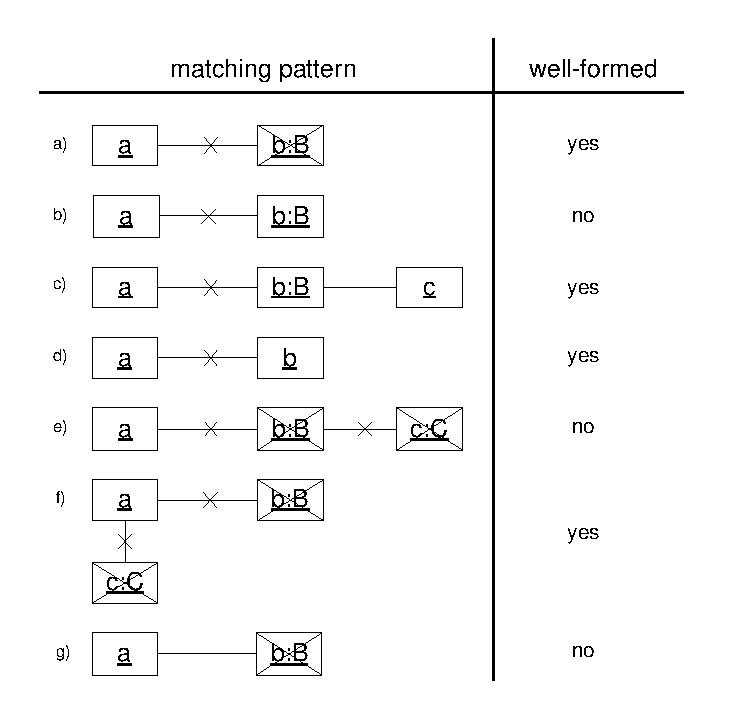
\includegraphics[scale=1]{figures/negativeObjects}
  \caption{Negative Application Conditions}
  \label{fig:negativeObjects}
\end{figure}

\todomcp{Optional objects, Figure \ref{fig:optionalObjects}:
the same as for negative objects?
a) allowed; same semantics for the same situation with link not optional?
b) not allowed because graph is not connected
c) allowed?
d) not allowed
e) allowed
f) allowed; same semantics for the same situation with links not optional
}

\begin{figure}[htbp]
  \centering
  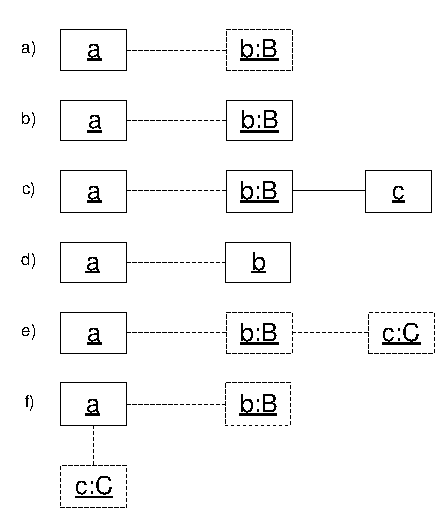
\includegraphics[scale=1]{figures/optionalObjects}
  \caption{Optional Objects}
  \label{fig:optionalObjects}
\end{figure}


\subsubsection{Feasible Binding Combinations}

\todomcp{check Table \ref{tab:bindingCombinations}}
% Table generated by Excel2LaTeX from sheet 'Tabelle1'
\begin{table}[htbp]
  \centering
  \caption{Feasible combinations of binding operators, binding states, and
  binding semantics for object variables}
    \begin{tabular}{|r|r|r|r|}
    \hline
    \textbf{Binding State} & \textbf{Binding Semantics} & \textbf{Binding
    Operator} & \textbf{Result} \\
    \hline
    UNBOUND & MANDATORY & CHECK\_ONLY & yes \\
    UNBOUND & MANDATORY & CREATE & yes \\
    UNBOUND & MANDATORY & DESTROY & yes \\
    UNBOUND & NEGATIVE & CHECK\_ONLY & yes \\
    UNBOUND & NEGATIVE & CREATE & no \\
    UNBOUND & NEGATIVE & DESTROY & no \\
    UNBOUND & OPTIONAL & CHECK\_ONLY & yes \\
    UNBOUND & OPTIONAL & CREATE & yes \\
    UNBOUND & OPTIONAL & DESTROY & yes \\
    \hline
    BOUND & MANDATORY & CHECK\_ONLY & yes \\
    BOUND & MANDATORY & CREATE & no \\
    BOUND & MANDATORY & DESTROY & yes \\
    BOUND & NEGATIVE & CHECK\_ONLY & no \\
    BOUND & NEGATIVE & CREATE & no \\
    BOUND & NEGATIVE & DESTROY & no \\
    BOUND & OPTIONAL & CHECK\_ONLY & no \\
    BOUND & OPTIONAL & CREATE & no \\
    BOUND & OPTIONAL & DESTROY & no \\
    \hline
    MAYBE\_BOUND & MANDATORY & CHECK\_ONLY & yes \\
    MAYBE\_BOUND & MANDATORY & CREATE & no \\
    MAYBE\_BOUND & MANDATORY & DESTROY & yes \\
    MAYBE\_BOUND & NEGATIVE & CHECK\_ONLY & no \\
    MAYBE\_BOUND & NEGATIVE & CREATE & no \\
    MAYBE\_BOUND & NEGATIVE & DESTROY & no \\
    MAYBE\_BOUND & OPTIONAL & CHECK\_ONLY & no \\
    MAYBE\_BOUND & OPTIONAL & CREATE & no \\
    MAYBE\_BOUND & OPTIONAL & DESTROY & no \\
    \hline
    \end{tabular}%
  \label{tab:bindingCombinations}%
\end{table}%

\todomcp{see albert's diss for example for optional-create}
\todomcp{table for link variables and for object set variables}

\subsection{Using Object Attributes [CH]}

object constraints, attribute assignments

\subsection{Object Sets [MCP]}

explain objectSetVariables, set size expressions

\todomcp{object sets and binding operators/states/semantics}

\todomcp{If we bind an object set, can we use the bound object in other story pattern? E.g. to insert all elements bound by the object set into a container via a containment link? (See Figure \ref{fig:reuseObjSet}).}
\tododt{Yes, but I would use another concrete syntax (see Figures~\ref{fig:reuseObjSet1}, \ref{fig:reuseObjSet2}, and \ref{fig:reuseObjSet1}).}

\begin{figure}[p]
	\begin{minipage}{.45\textwidth}
		\centering
		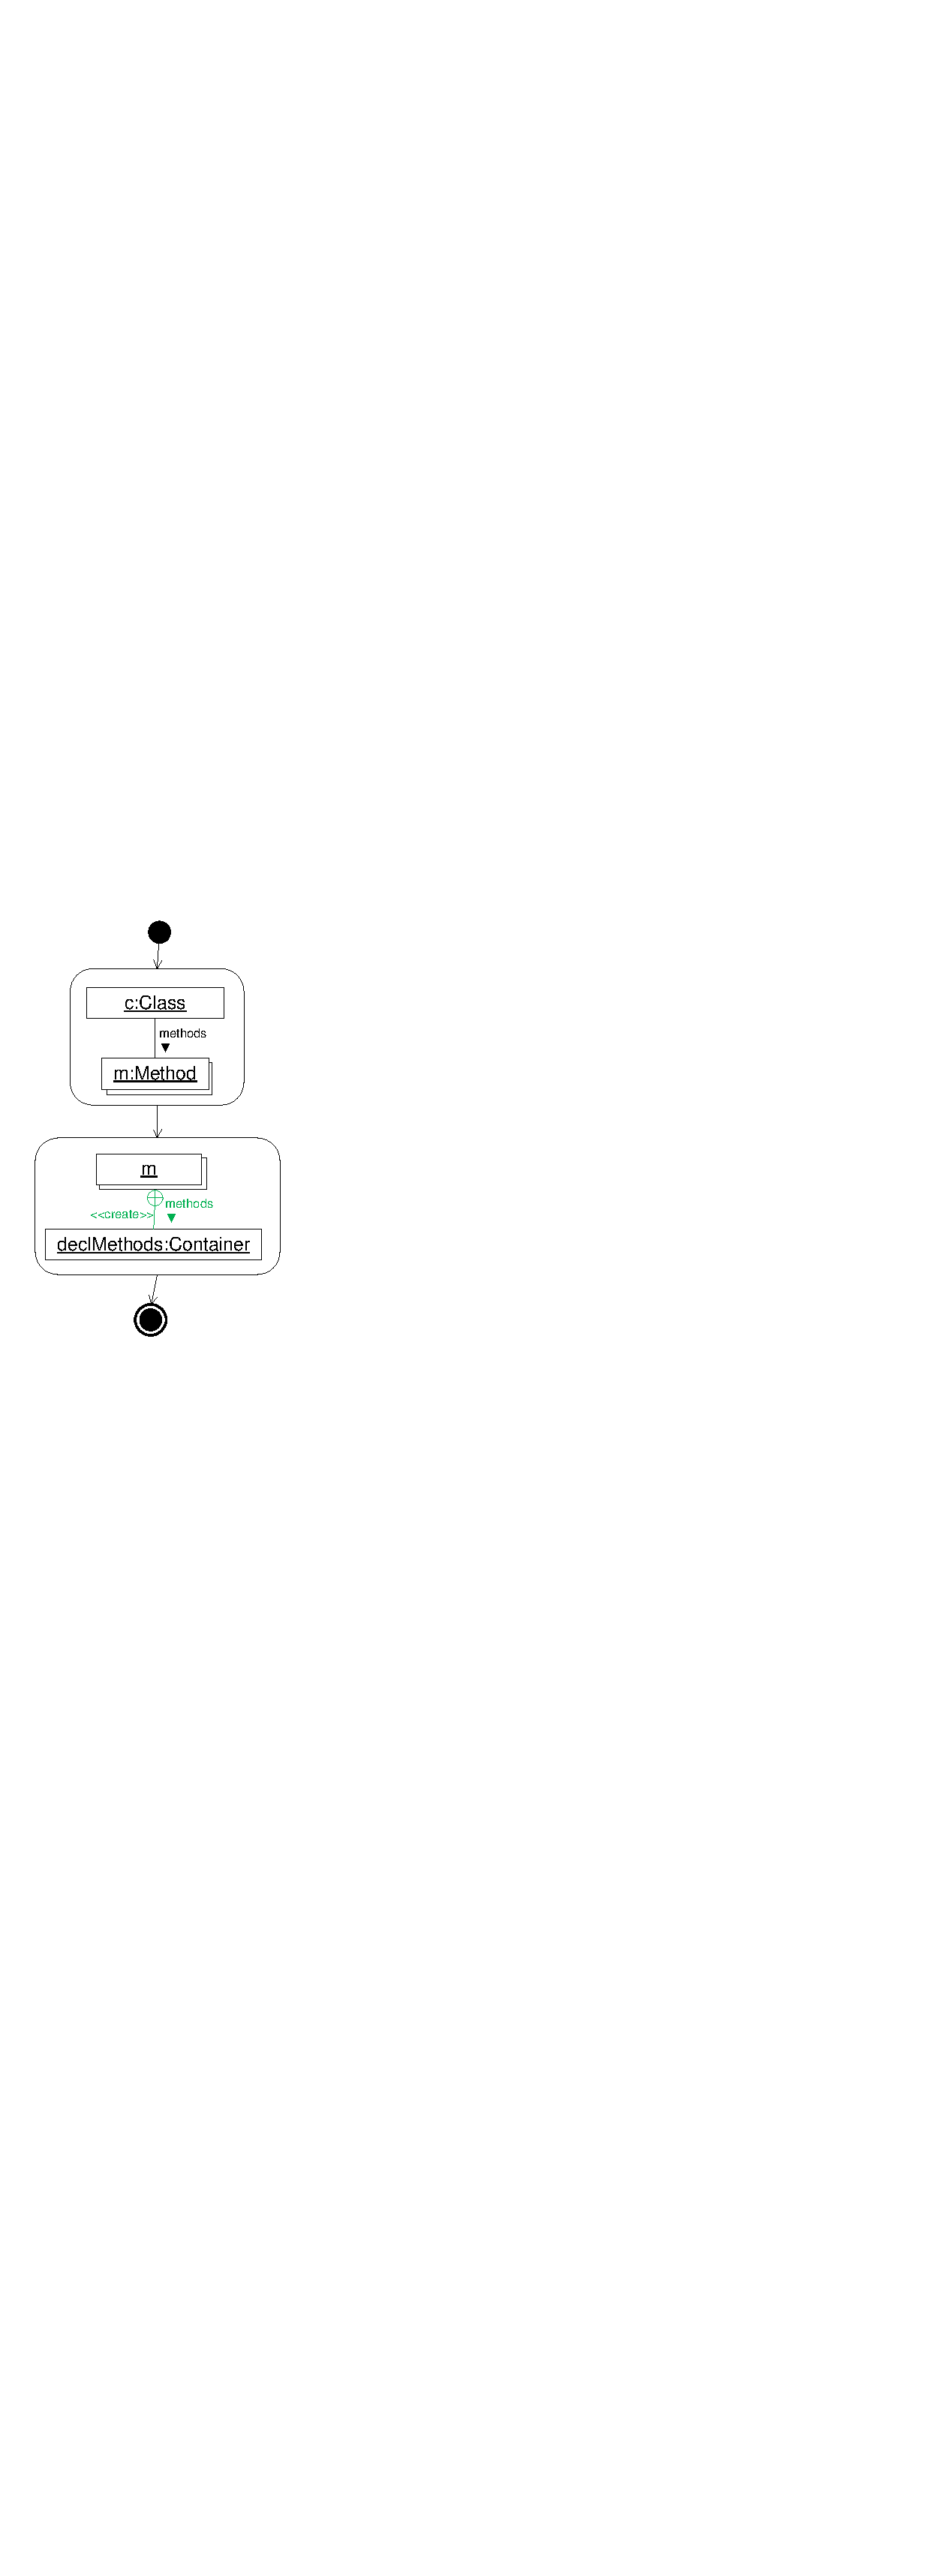
\includegraphics[scale=.8]{figures/ReuseObjectSet}
  	\caption{Reusing Object Sets}
  	\label{fig:reuseObjSet}
	\end{minipage}
  \hfill
  \begin{minipage}{.45\textwidth}
  	\centering
		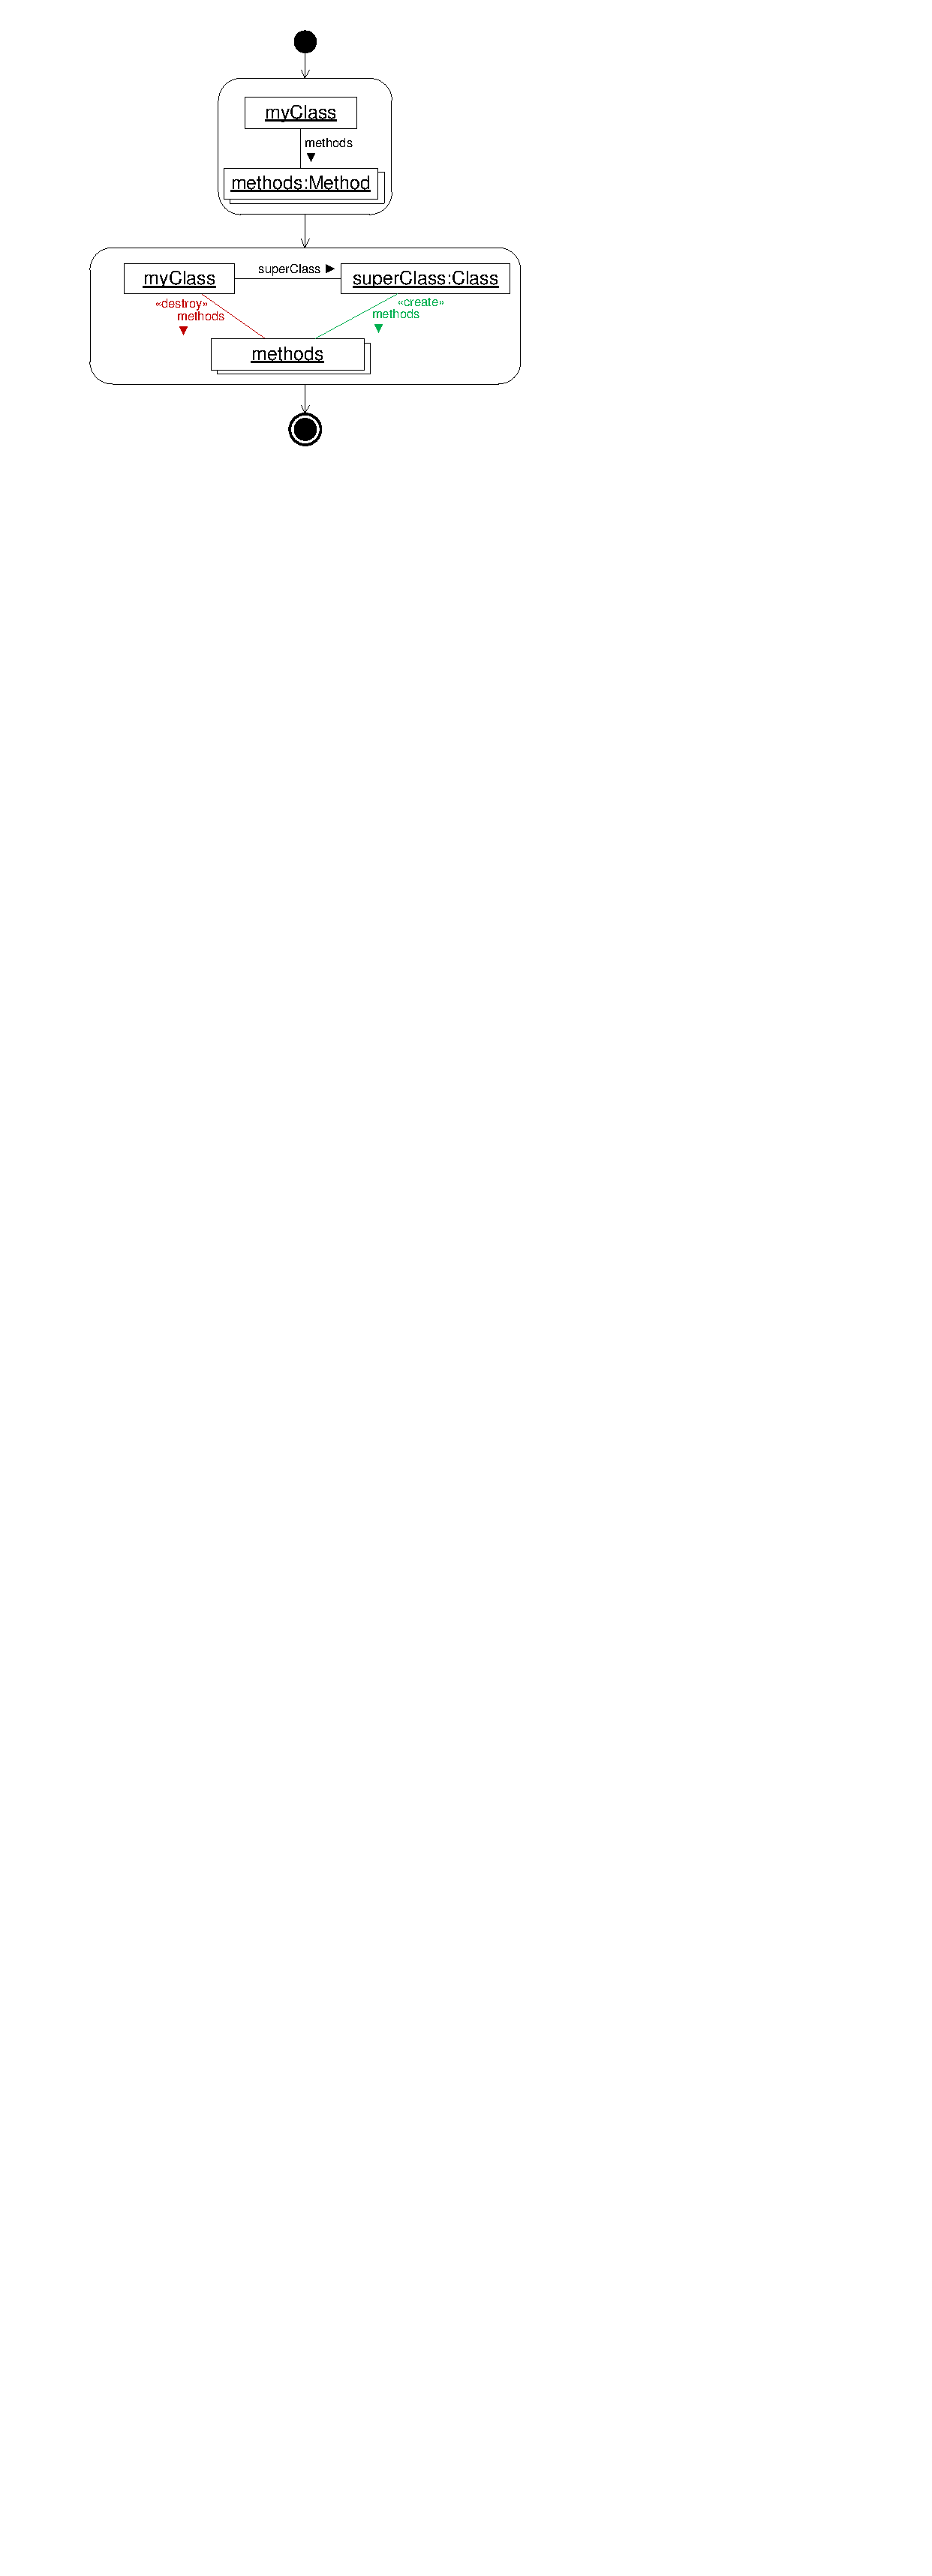
\includegraphics[scale=.8]{figures/ReuseObjectSet1}
  	\caption{Reuse objects in a set}
  	\label{fig:reuseObjSet1}
	\end{minipage}
\end{figure}

\begin{figure}[p]
	\begin{minipage}{.45\textwidth}
		\centering
		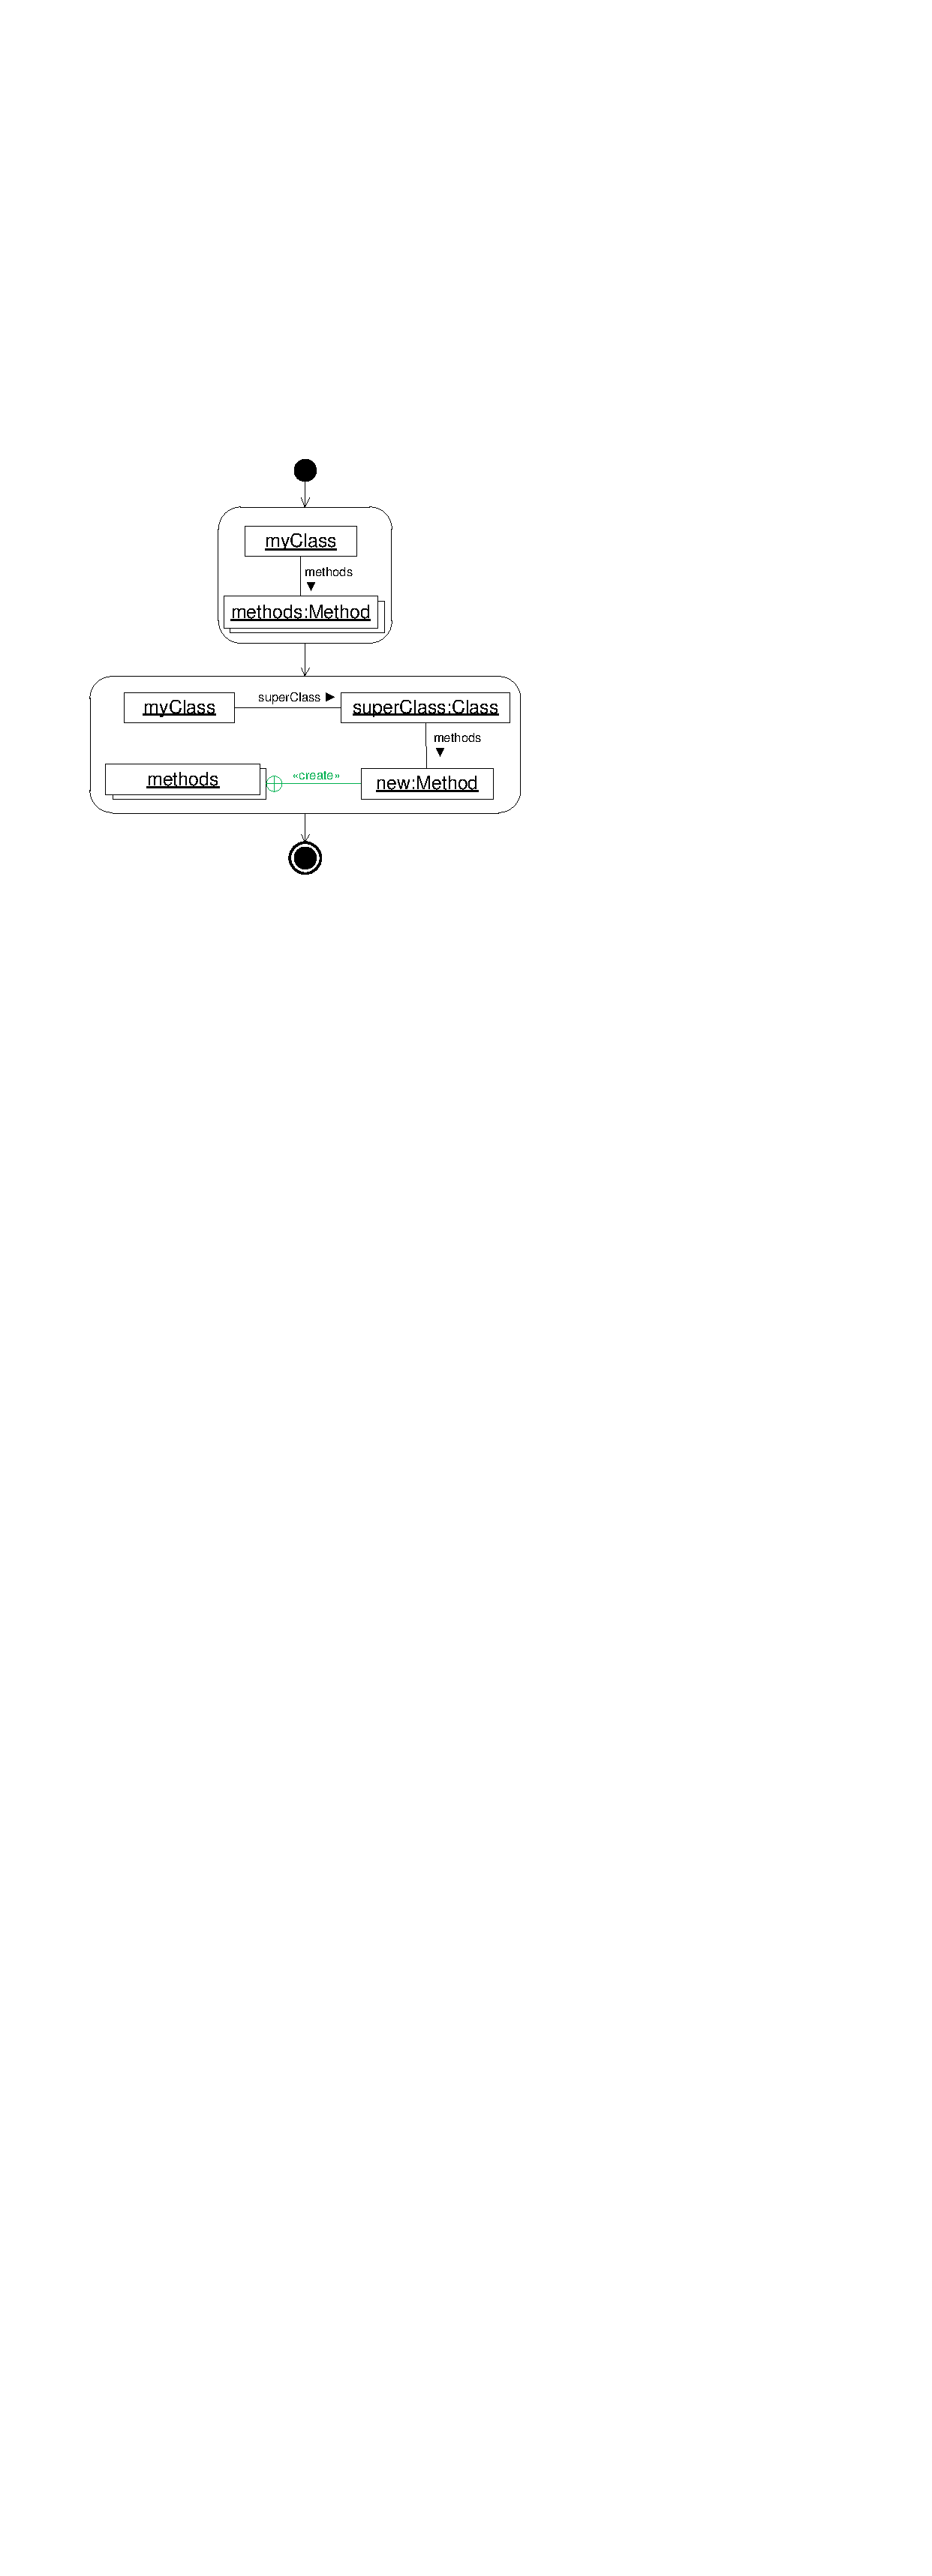
\includegraphics[scale=.8]{figures/ReuseObjectSet2}
  	\caption{Add an object to a set}
  	\label{fig:reuseObjSet2}
	\end{minipage}
  \hfill
  \begin{minipage}{.45\textwidth}
  	\centering
		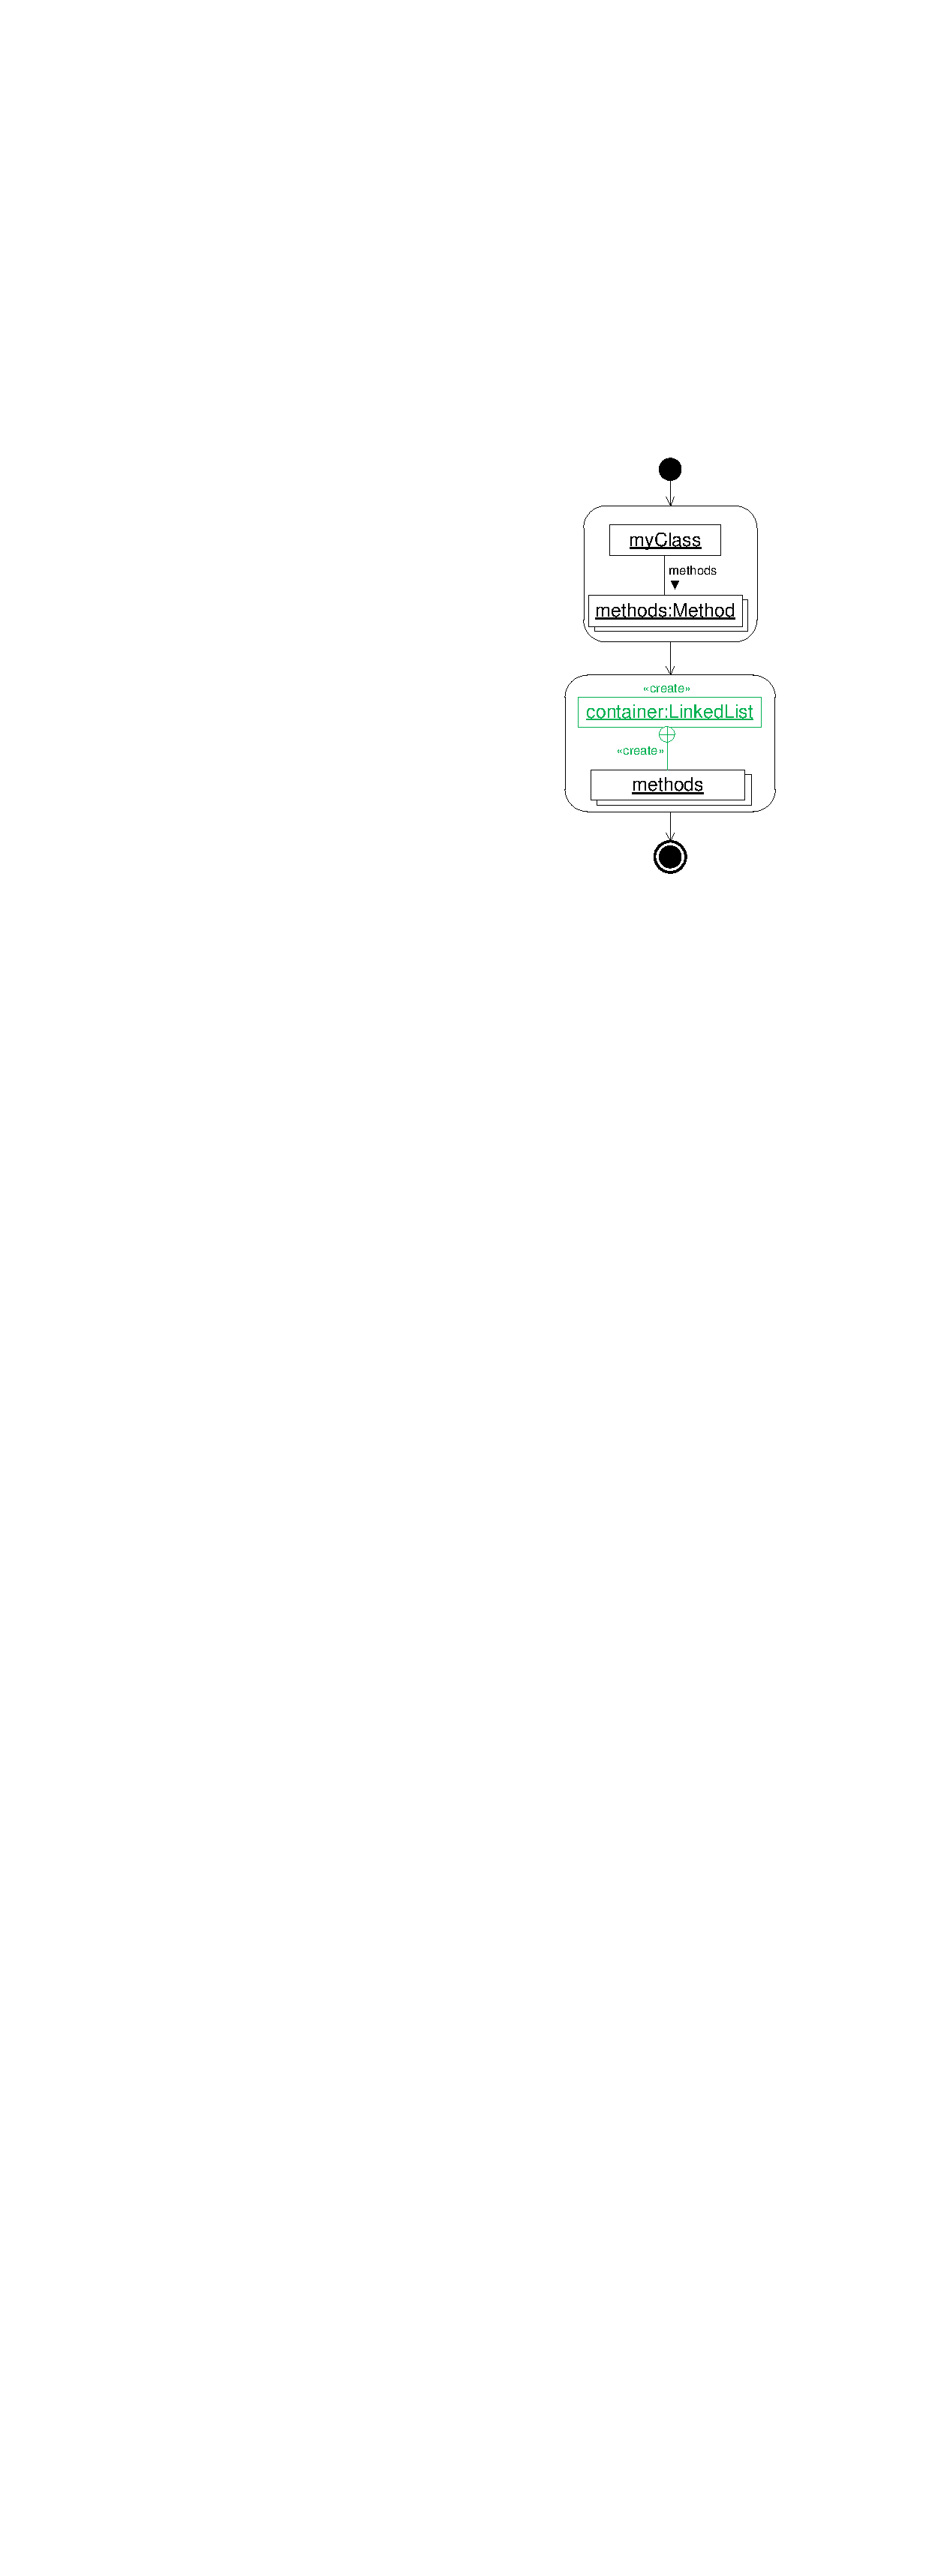
\includegraphics[scale=.8]{figures/ReuseObjectSet3}
  	\caption{Add all objects from a set to a container}
  	\label{fig:reuseObjSet3}
	\end{minipage}
\end{figure}

\todomcp{An object set contains no ObjectSetSizeExpression and no object is matched into the object set: ObjectSet is interpreted as optional and the matching succeeds.}

\todomcp{All operators for comparison are allowed: <, <=, >, >=, = !=}


\begin{figure}[p]
	\begin{minipage}{.45\textwidth}
		\centering
		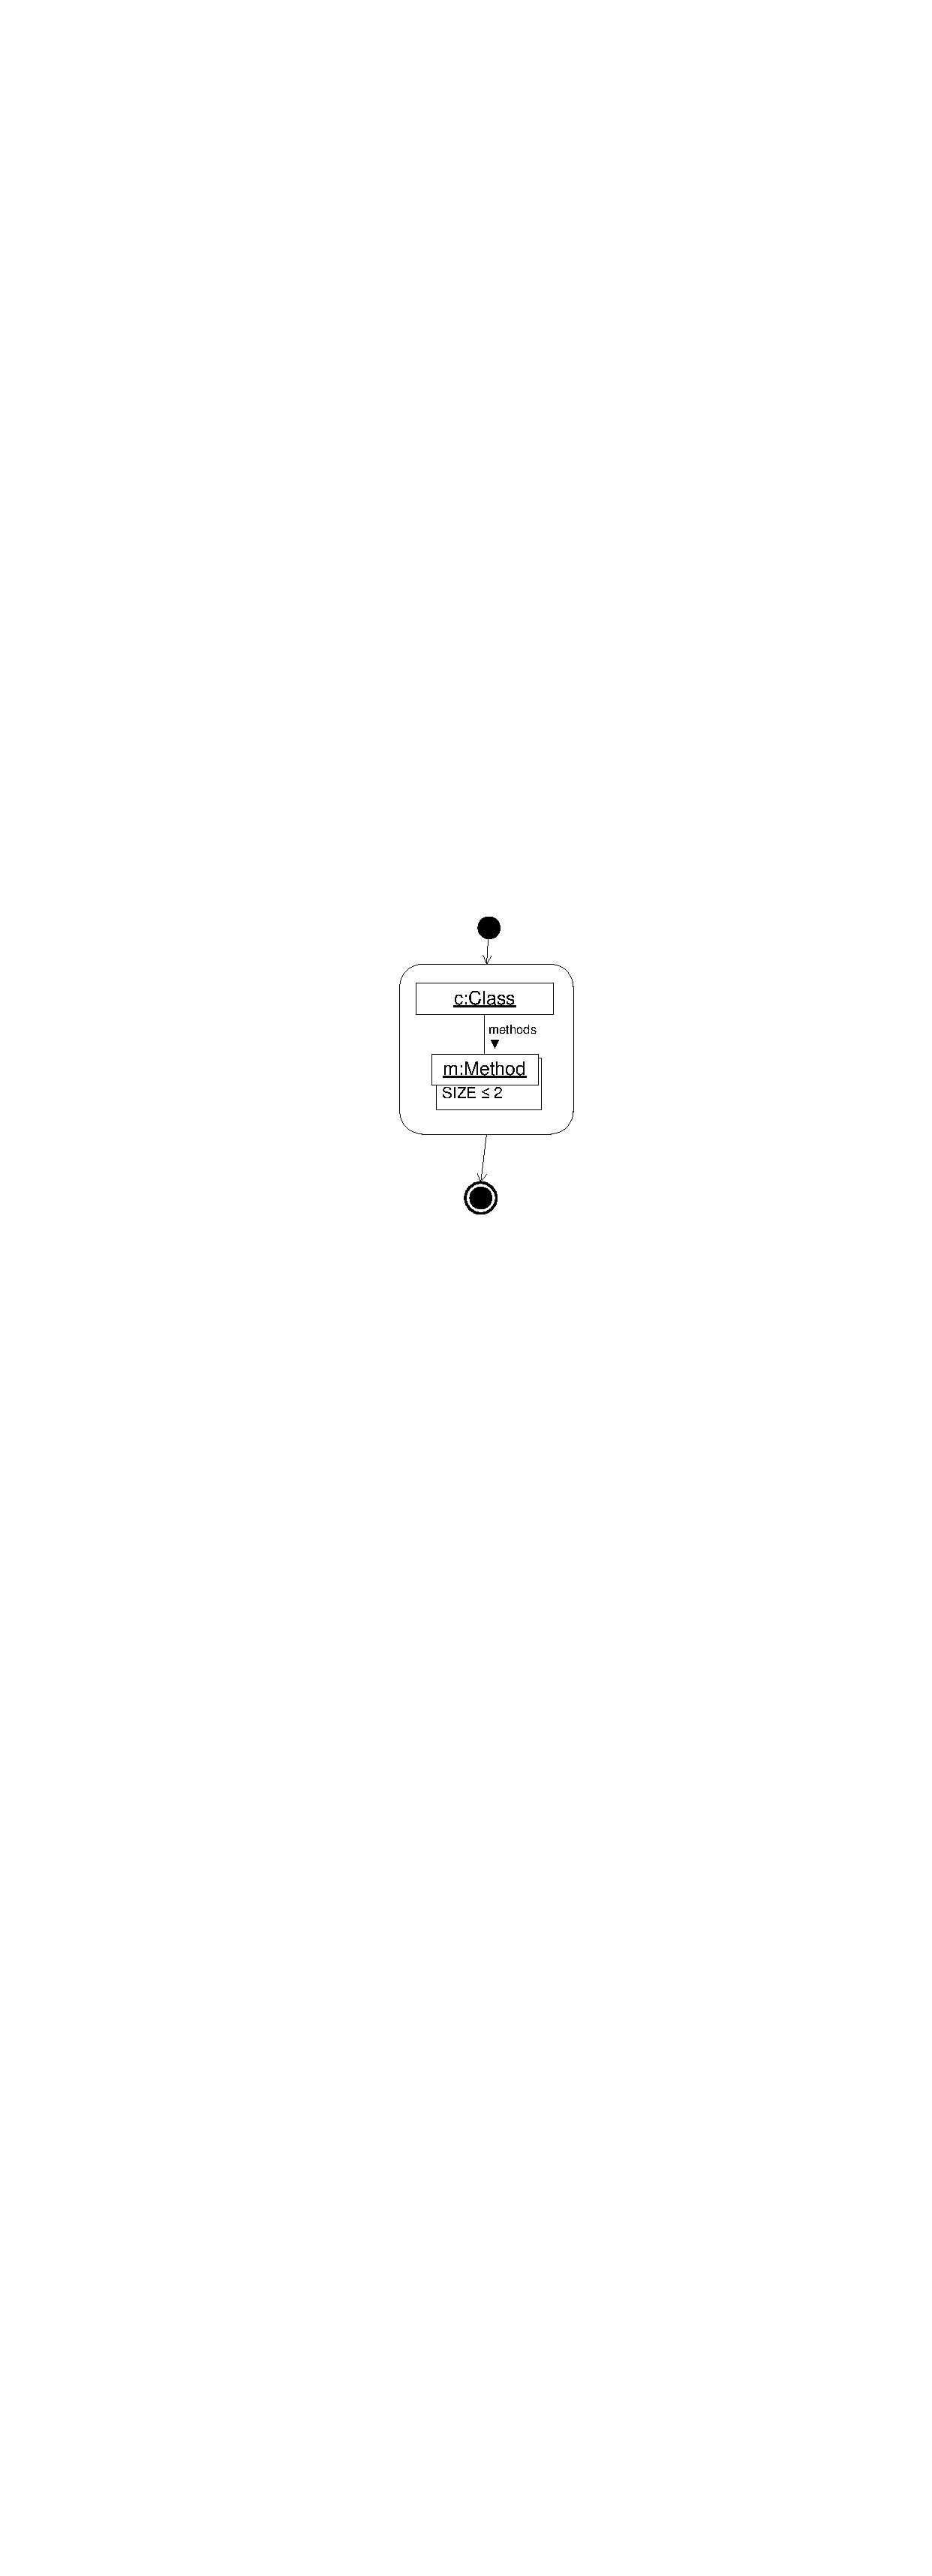
\includegraphics[scale=.8]{figures/ObjectSetSize}
  	\caption{Object Set Size}
  	\label{fig:objSetSize}
	\end{minipage}
  \hfill
  \begin{minipage}{.45\textwidth}
  	\centering
		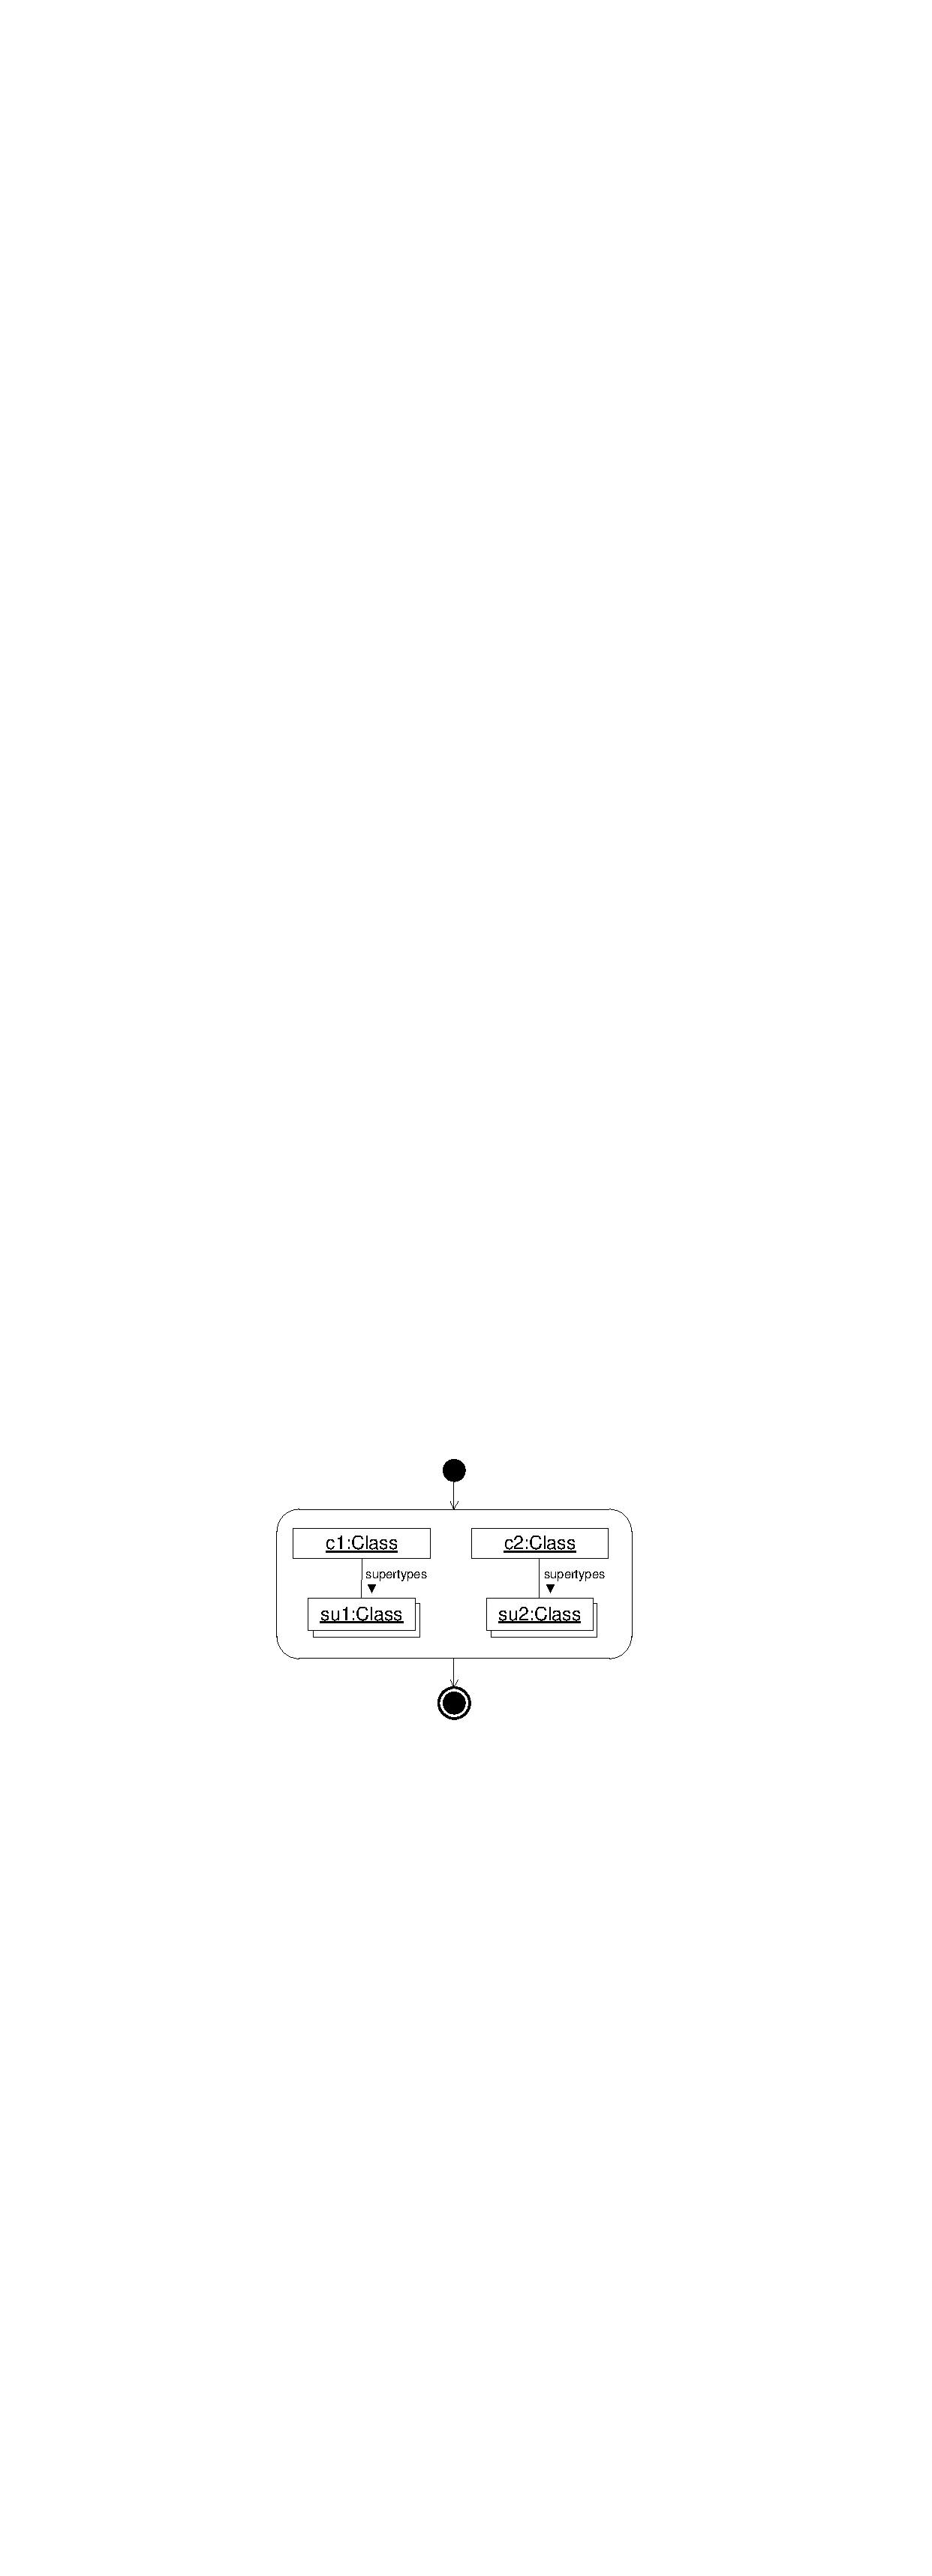
\includegraphics[scale=.8]{figures/IsomorphismInObjectSets}
  	\caption{Isomorphism in Object Sets}
  	\label{fig:isoObjSet}
	\end{minipage}
\end{figure}

\todomcp{What happens if one pattern contains two object sets that may possibly contain the same objects. Consider the pattern in Figure \ref{fig:isoObjSet}. If c1 and c2 share the same super classes, su1 and su2 contain the same objects. Is this allowed? Isomorphic matching would normally forbid this.}

\tododt{I would allow this which would comply with our isomorphic matching.
But in this case it is non-deterministic how the objects are matched to the set nodes (assuming the classes are already bound).
A maybe constraint could allow to match the same objects to both sets.}
\todojr{We decided to match set nodes without them having to be disjoint, thus, we do not enforce isomorphism for the content of two or more set variables.}

\subsection{Special Link Kinds [CH]}

\subsubsection{Inclusion Links [CH]}

\todoch{What is the semantics of a containment link? Current understanding: an element is contained in a container. What is the difference to to-many references which are containments?}
\tododt{Containment links do not correspond to any association or reference. They only describe containments of objects in containers or set nodes.}

\todoch{Which classifiers are allowed for ContainerVariables? This should not only be the EMF collection types EList and EMap. Does a ContainmentLink need a reference as a type like normal LinkVariables?}
\tododt{The contaiment links do not need any reference. I would suggest to allow any subtype of java.util.Collection (and java.util.List in case that link order constraints are used), but not java.util.Map! This is something different and needs a key for containment. Maybe we need special containment links for maps that include a key.}

\subsubsection{Paths [MCP]}

\subsubsection{Link Constraints [CH]}

\todoch{What is the concrete Syntax for this?}

\tododt{I have a suggestion in Figure~\ref{fig:linkConstraints}.}

\begin{figure}[p]
  \centering
  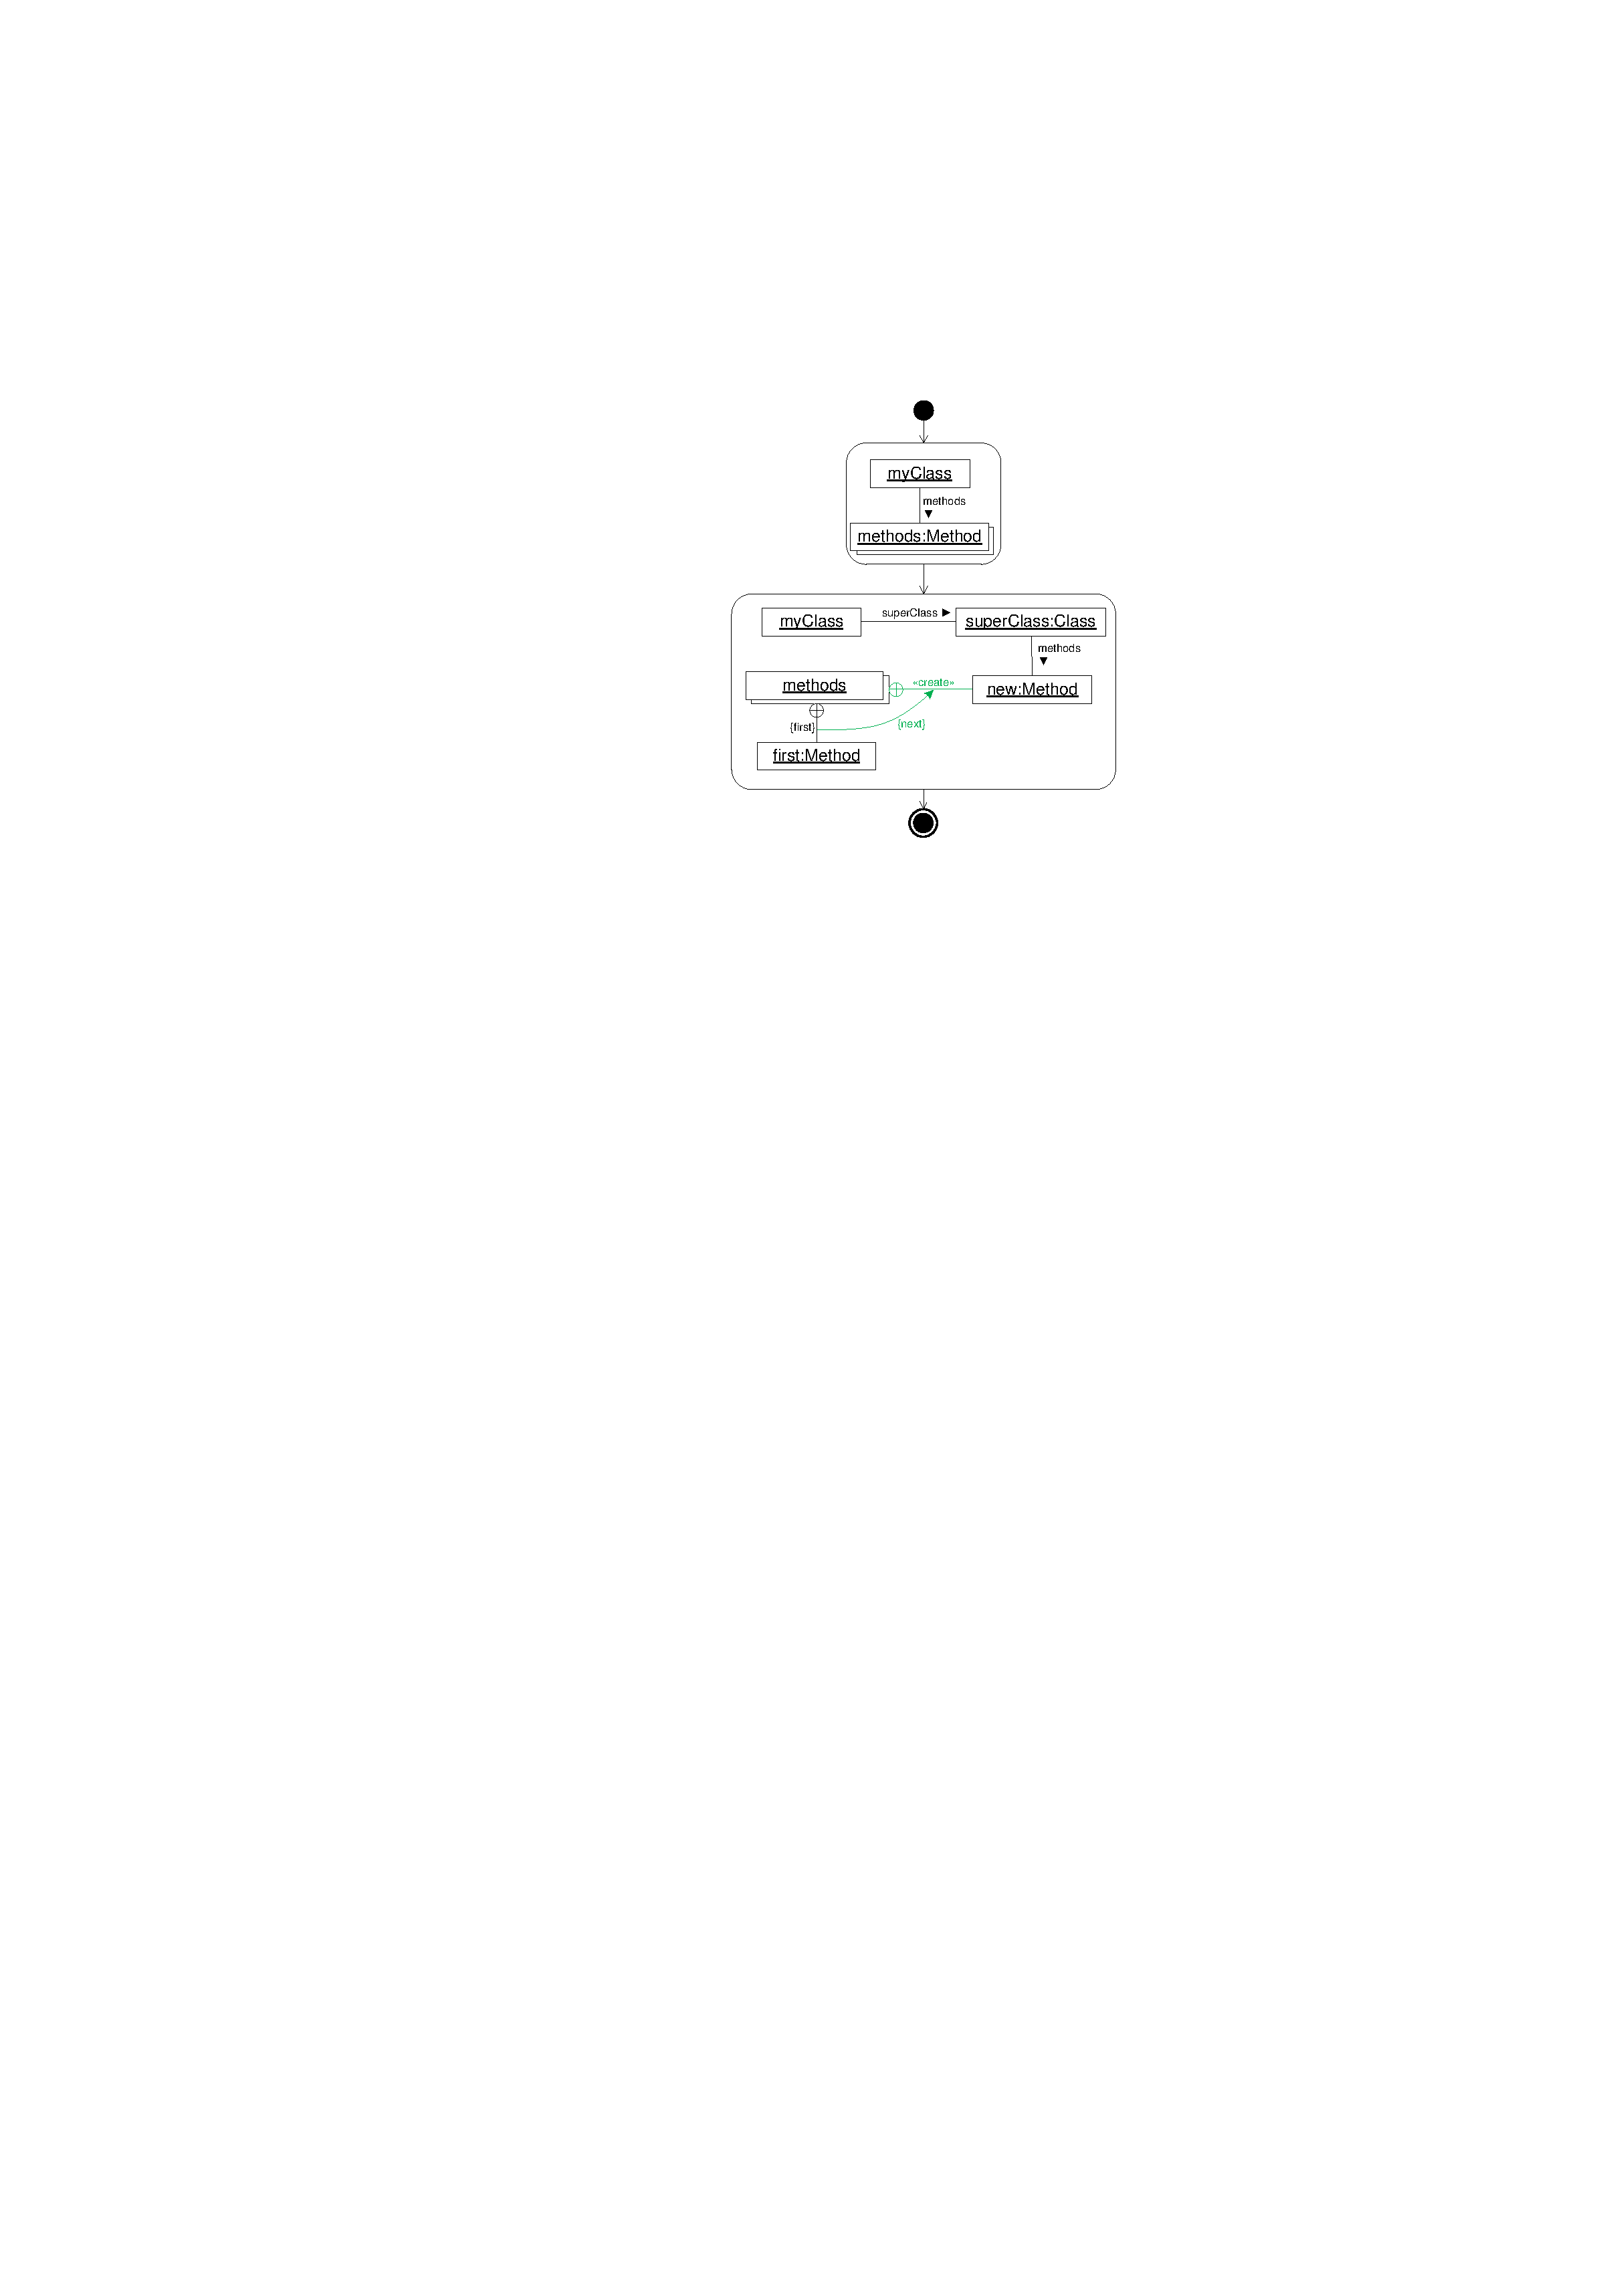
\includegraphics[scale=.8]{figures/LinkConstraints1}
  \caption{Link order constraints FIRST and DIRECT\_SUCCESSOR}
  \label{fig:linkConstraints}
\end{figure}

Link constraints are only applicable to link variables that reference an ordered to-many reference.
\todoch{No link constraints for inclusion links.}

\begin{itemize}
  \item FIRST = matches the first element in the list, requires one link variable
  \item LAST = matches the last element in the list, requires one link variable
%  \item INDEX = matches the element at the specified index, requires one link variable
%  \todoch{Our lowest index value is 0, not 1.}
  \item DIRECT\_SUCCESSOR = requires two link variables, target of the second one must be located directly after the target of the first one in the list
  \item SUCCESSOR = requires two link variables, target of the second one must be located somewhere after the target of the first one in the list
\end{itemize}

\todojr{We will separate link constraints for single links and those for two links and their order. Stephan will make a suggestion.}

\todoch{Is this semantic description correct/complete?}

\subsubsection{Maybe Links}

Disables the isomorphism check for two object variables, these two object variables may be matched to the same object.

\todoch{What is the concrete Syntax? Using a special pattern constraint as proposed in Alberts Habil is very low-level. Alternative version is proposed in Figure \ref{fig:maybeLink}.}
\todoch{conrete syntax: "same?"}

\begin{figure}[htbp]
  \centering
  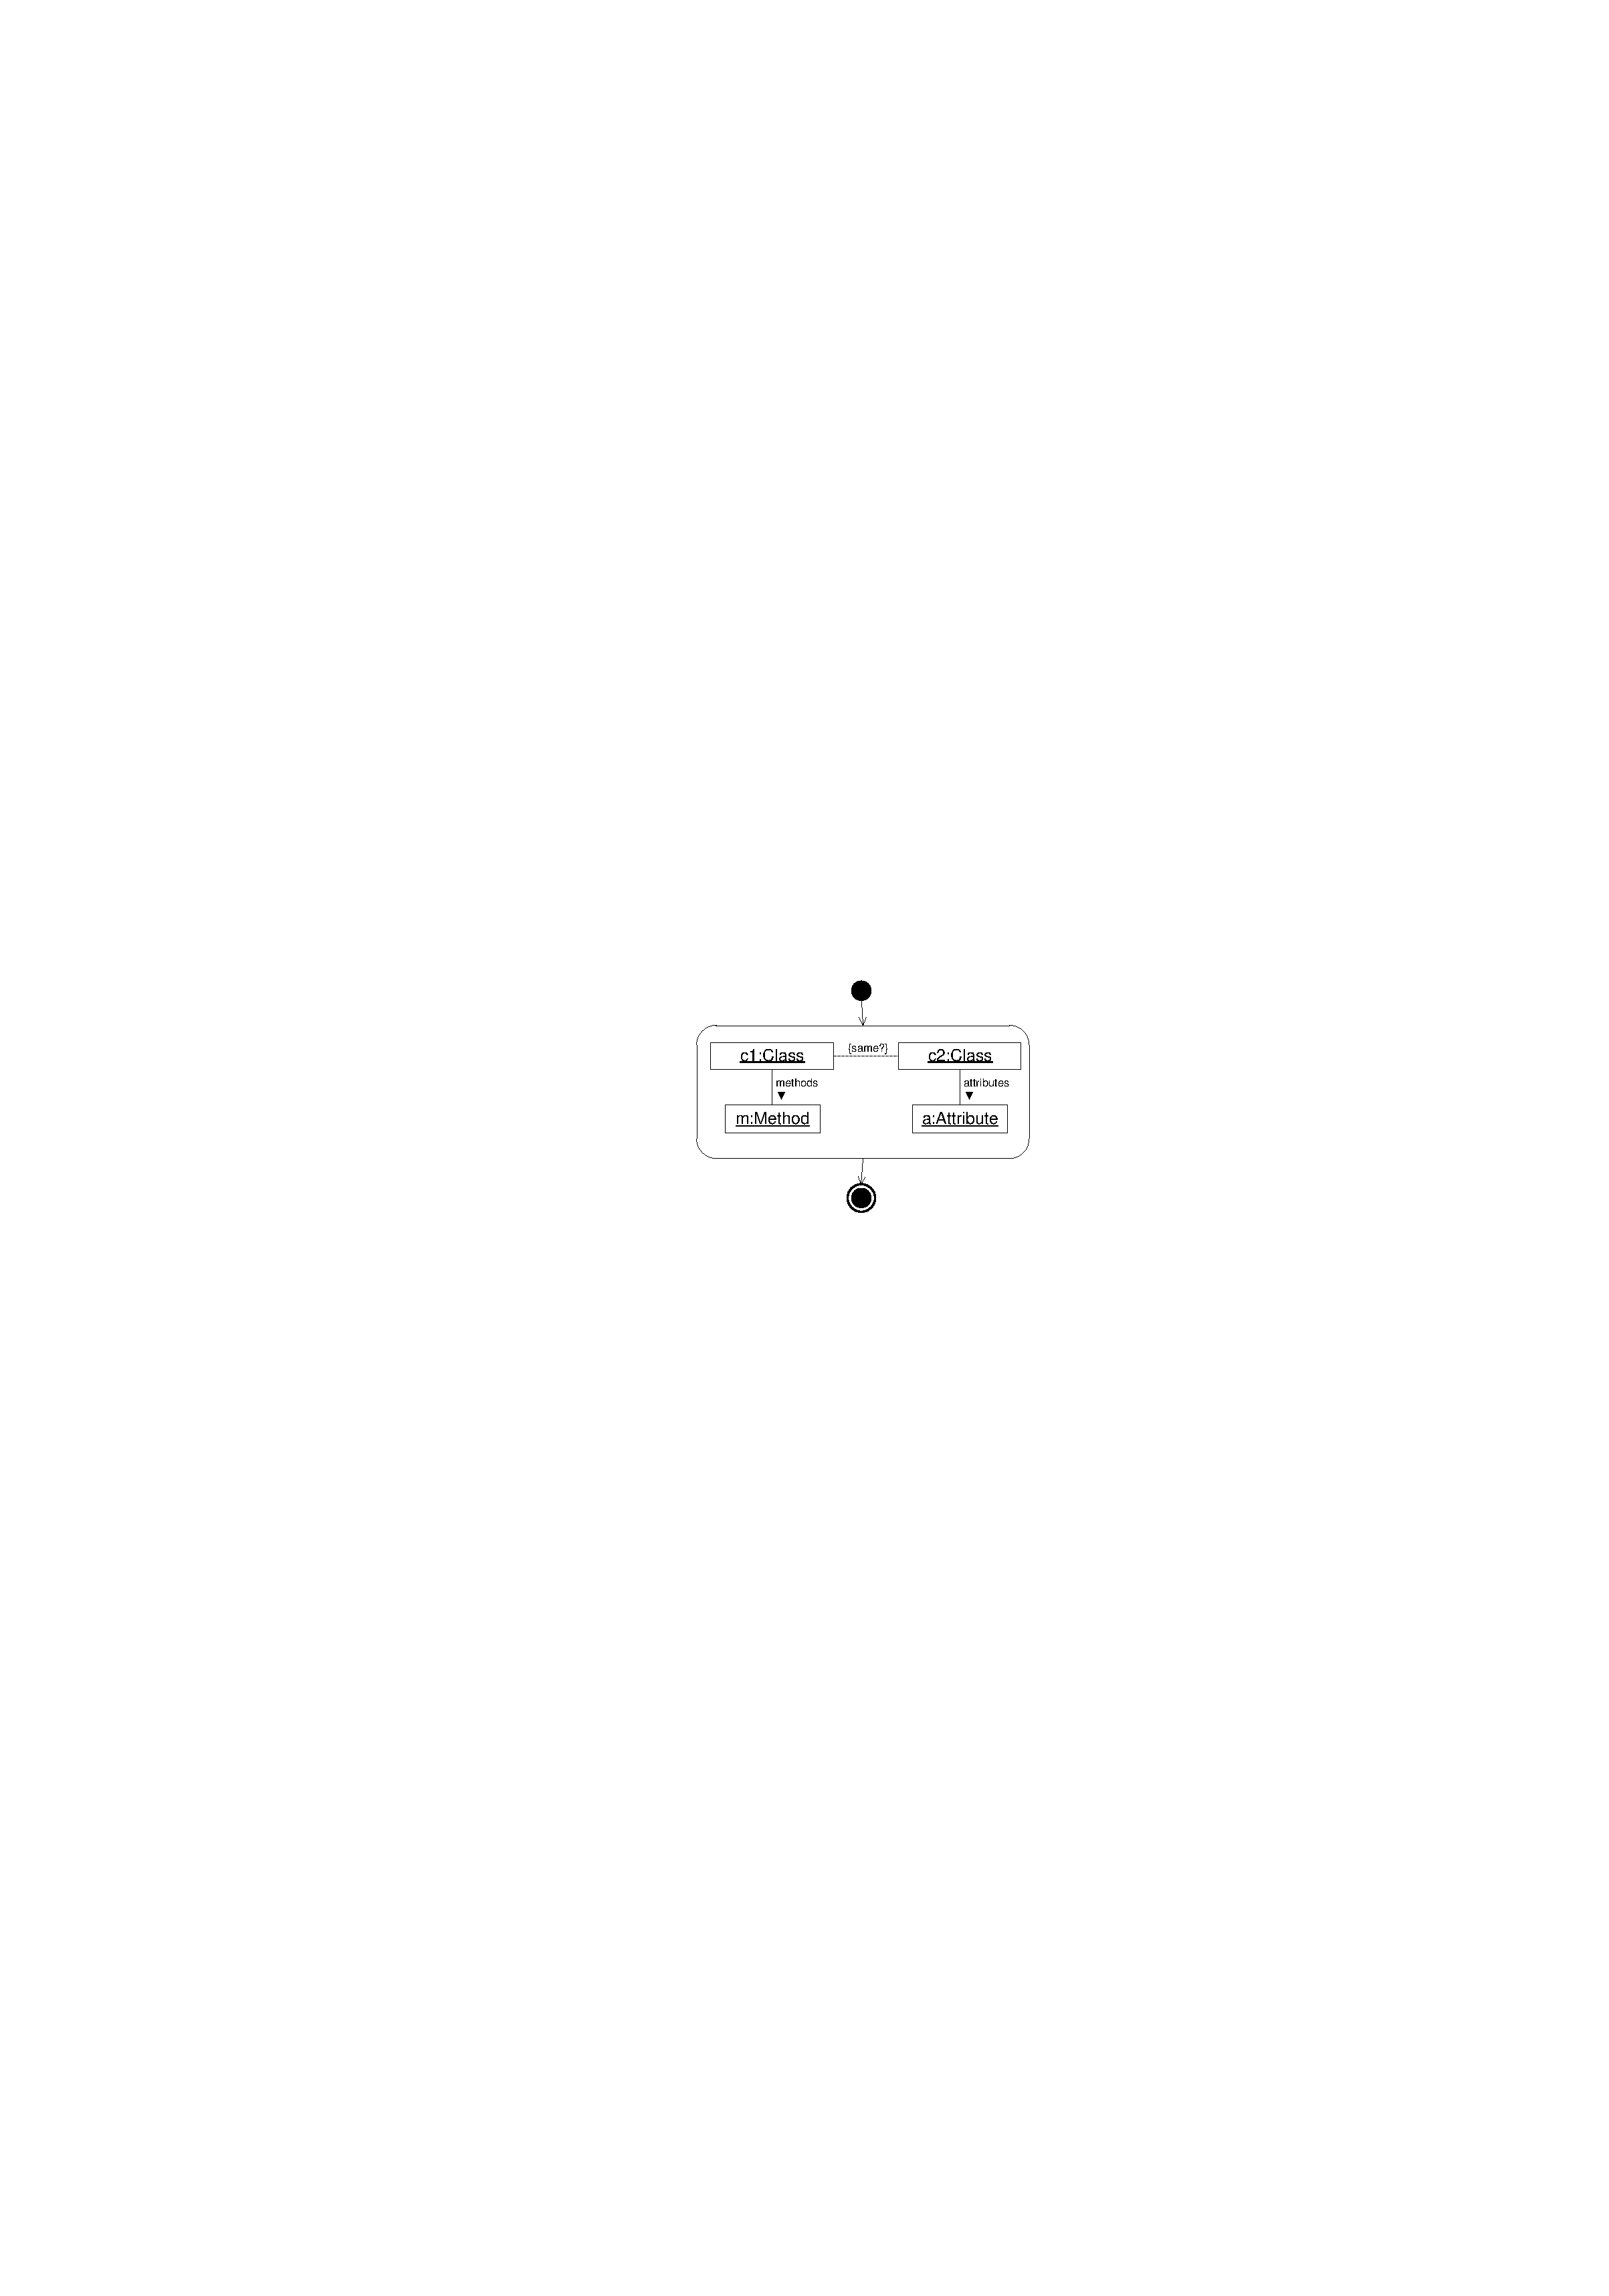
\includegraphics[scale=.8]{figures/MaybeLink}
  \caption{Maybe Link}
  \label{fig:maybeLink}
\end{figure}

\subsection{Pattern Constraints [CH]}

\todoch{What happens when a pattern constraint is placed inside a for each story pattern (not inside a node in that pattern)? Proposal: The particular match must fulfill the pattern constraint, if it does not fulfill the pattern constraint, the match is rejected and the iteration continues.}
\tododt{Exactly. In this case, it is a kind of post condition that has to be satisfied at the end of the matching step.}

\subsection{Pattern Fragments [MCP]}

patterns contained in other patterns, negative, semantics? review enhanced story patterns from Diss Florian Klein

\todomcp{Should contained pattern be marked as forEach? Idea for semantics: first the part of the pattern outside the forEach pattern is matched, then the forEach subpattern is applied to any match that may be located, the variables bound in a forEach subpattern may not be used in subsequent activities}

\tododt{This is somewhat confusing.
As I understand them, subpatterns are ordinary story patterns within another story pattern.
They are surrounded by a fragment box and can be labeled with a name (see Figure~\ref{fig:labeledSubPattern}).
Special types of such subpatterns are negative application condition fragments (NACs), set fragments, and optional fragments.
As far as I know, we did not plan to add $\forall$ and $\exists$ fragments, did we?
These are only used in SDDs and TSSDs which are constraint languages.
}

\begin{figure}[htbp]
  \centering
  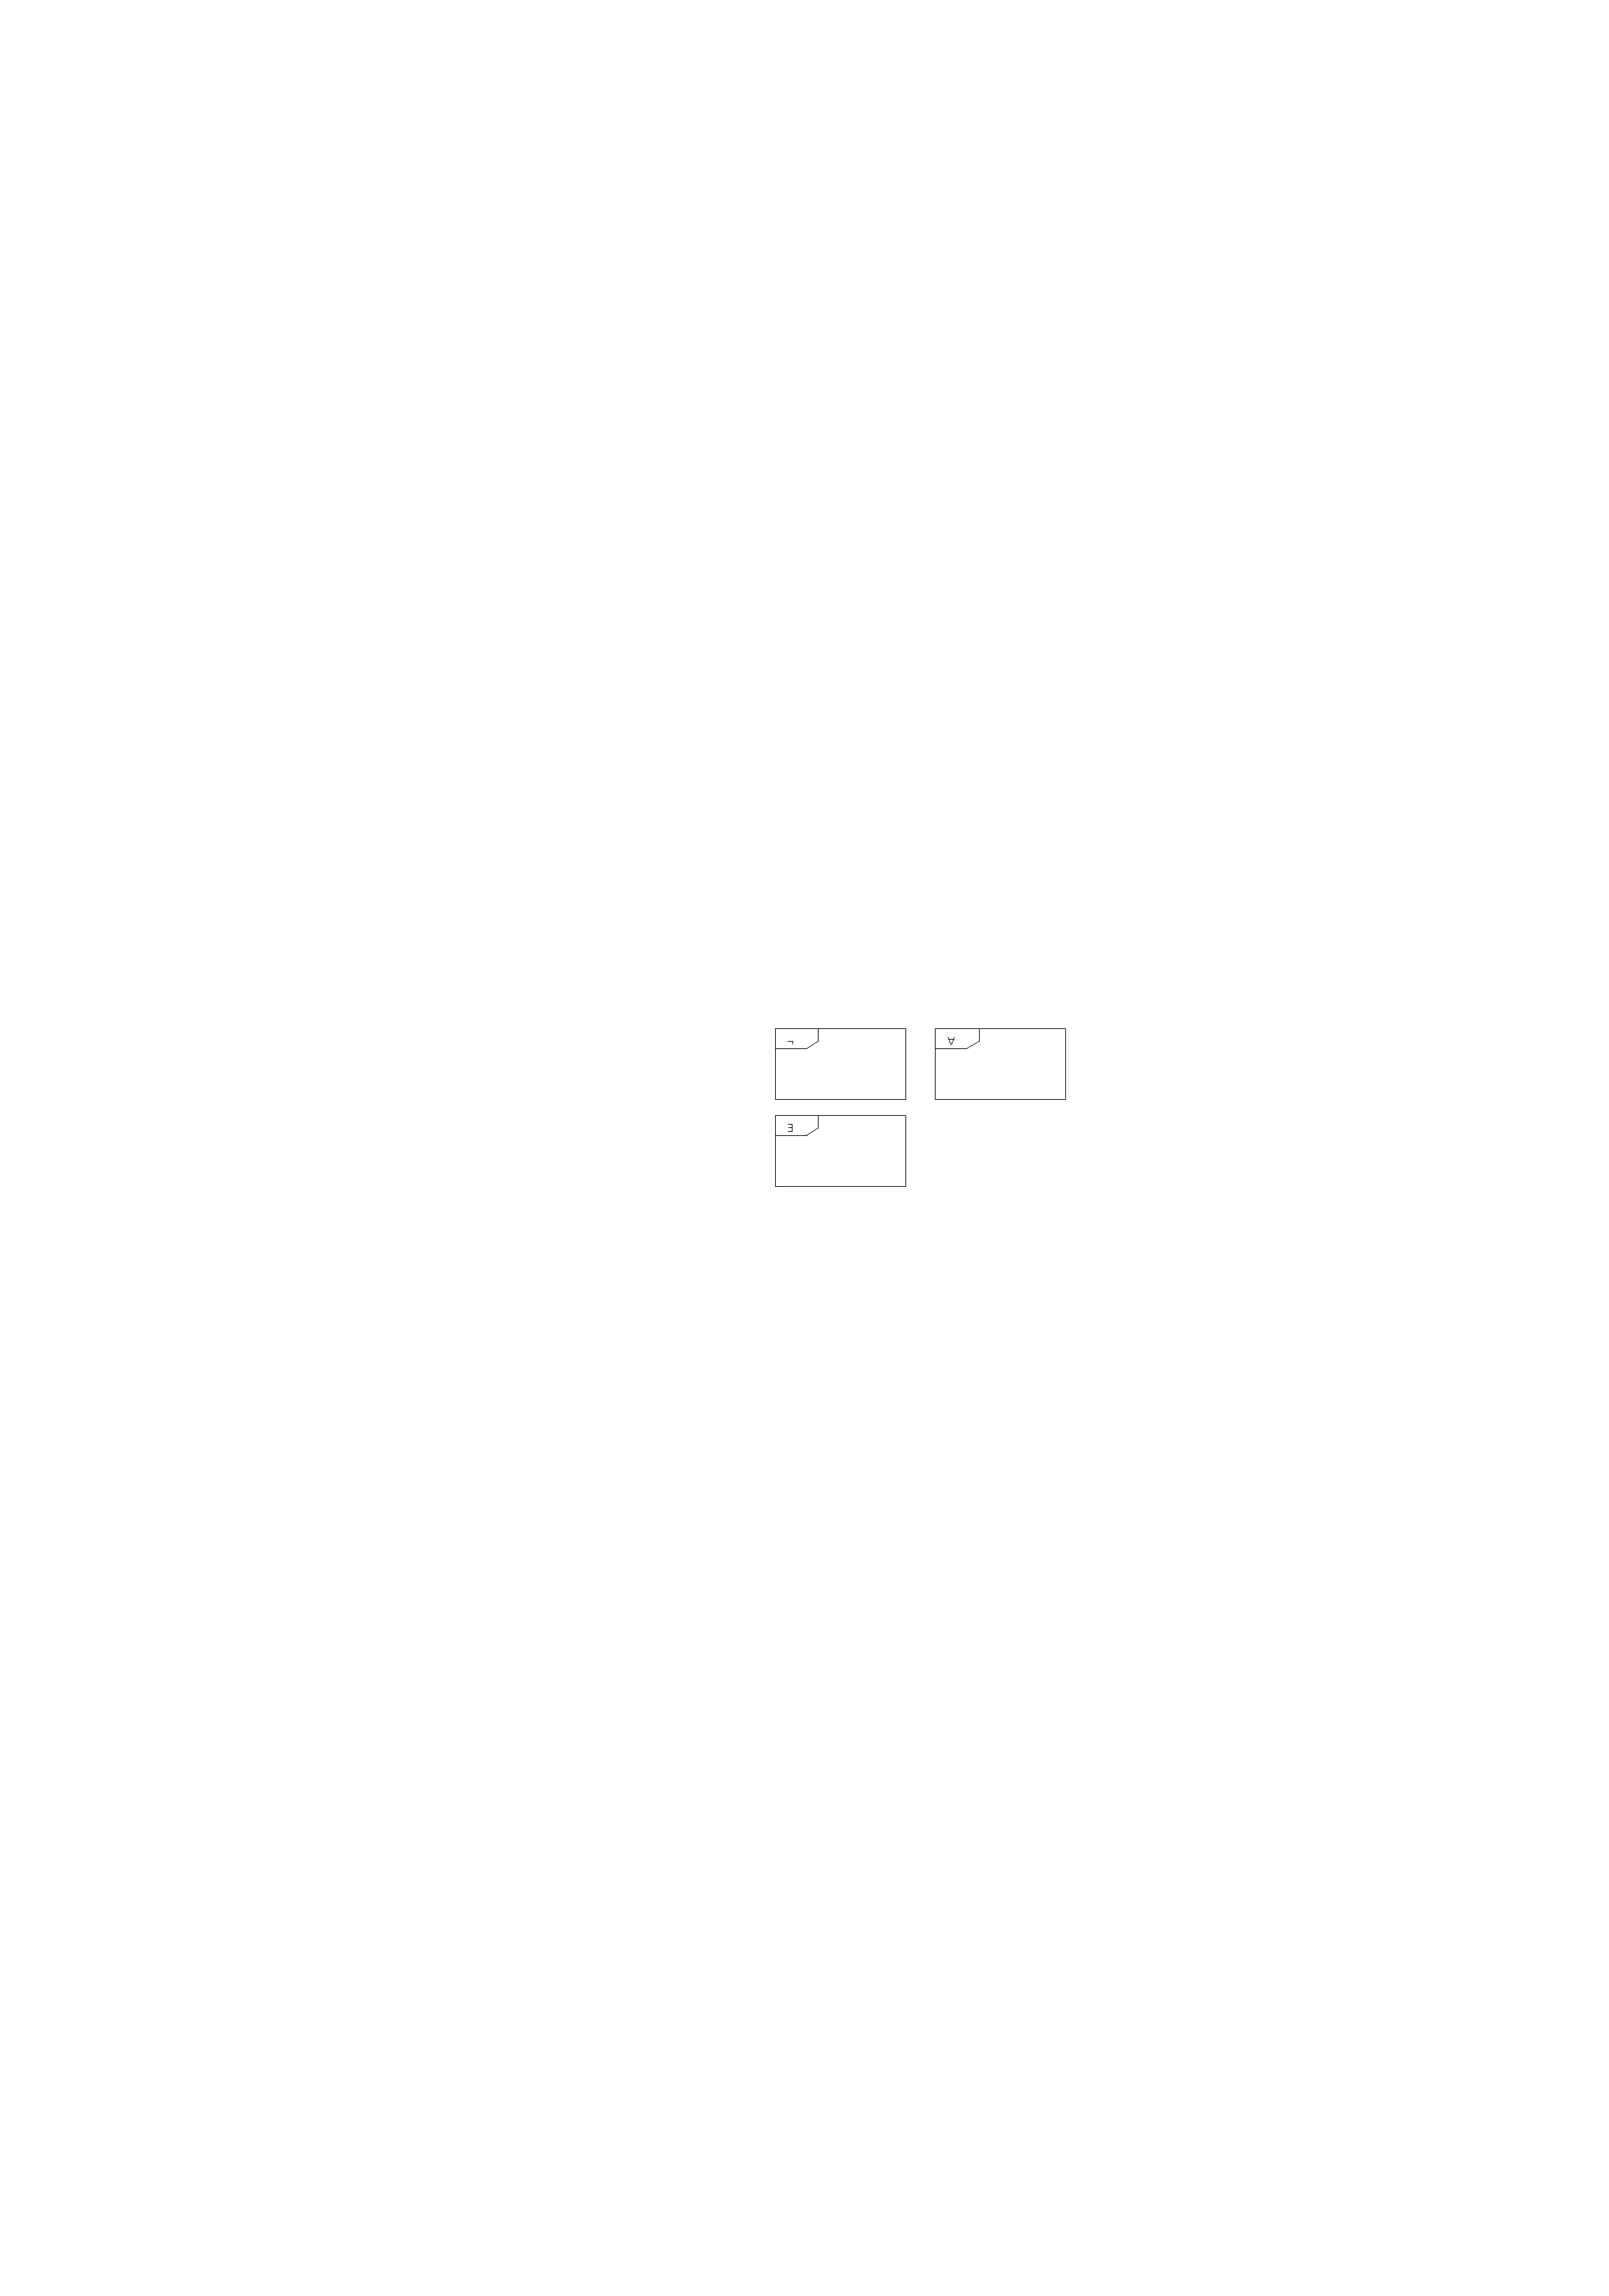
\includegraphics[scale=1.0]{figures/ContainedPattern}
  \caption{Different Kinds of Contained Patterns}
  \label{fig:containedPattern}
\end{figure}

\todomcp{Should contained pattern be marked as optional? Is currently possible in the meta-model. Idea for semantics: Whole pattern must be found, if found, variables may be used in subsequent activities, if pattern may not be found as a whole, matching still succeeds but all variables in the subpattern are not bound in subsequent activities.}
\tododt{I would say, contained patterns are mandatory in general (or are NAC/optional/set in case of the according fragment).}

\begin{figure}[htbp]
  \centering
  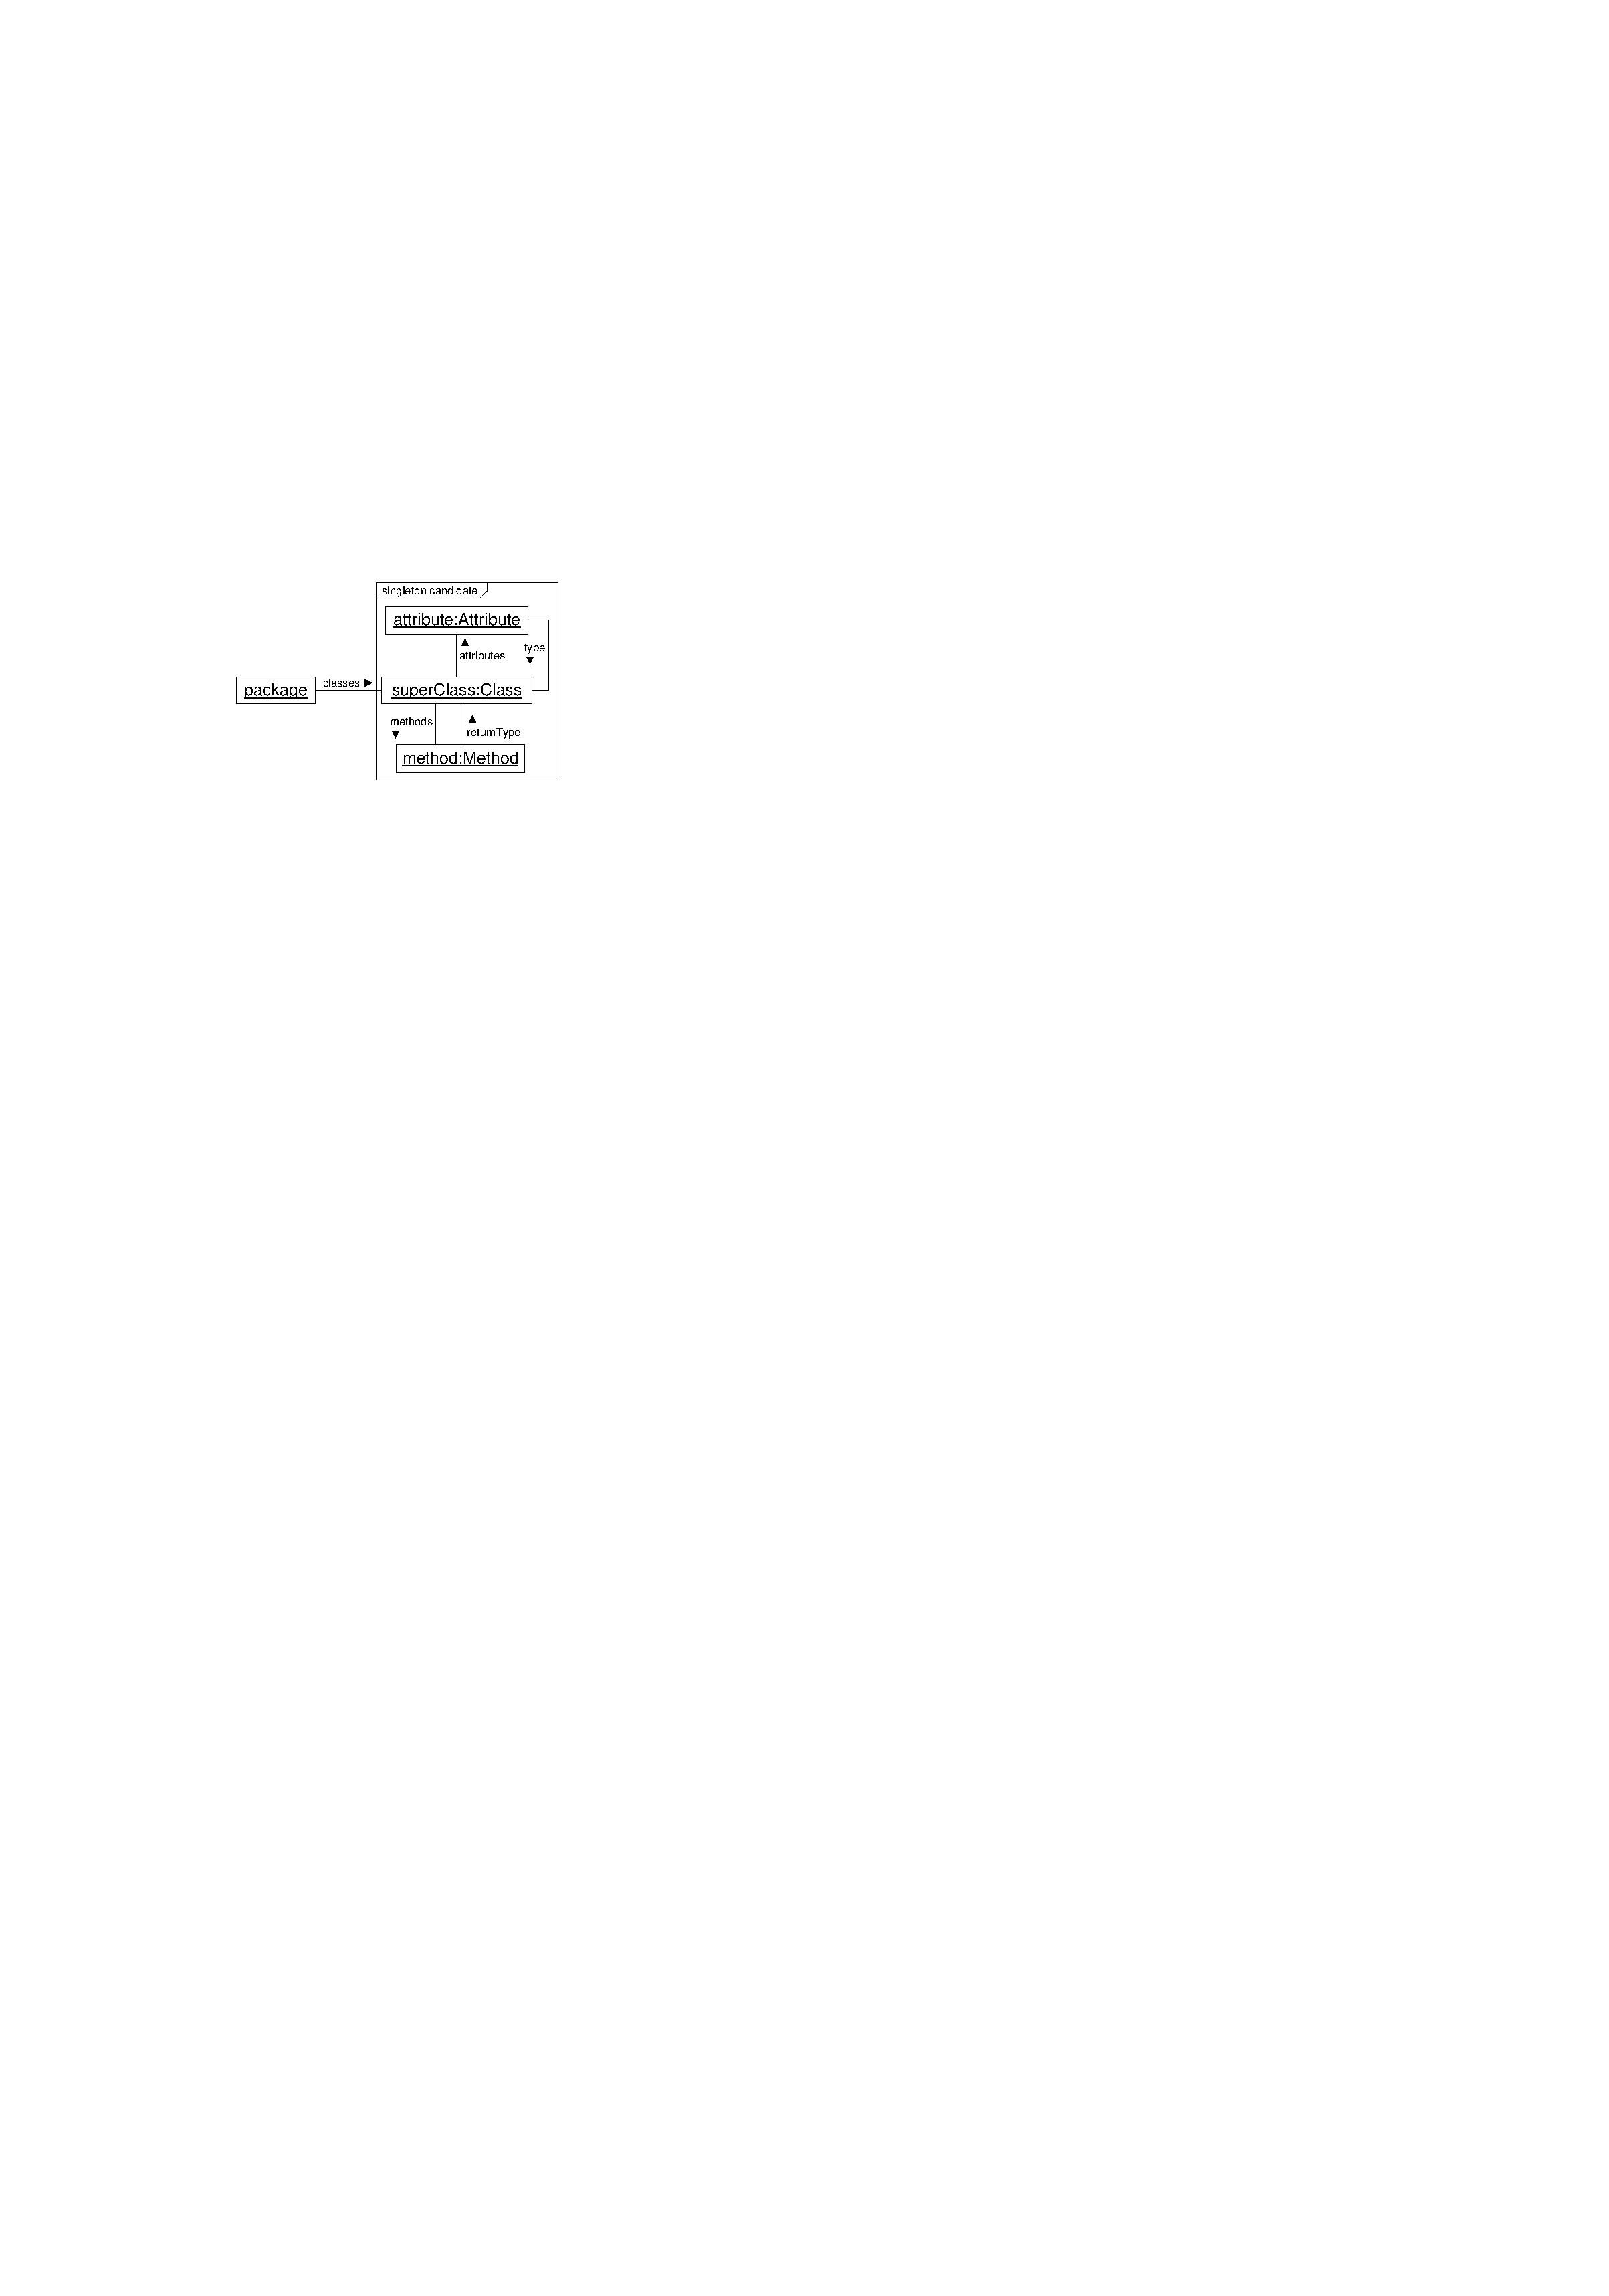
\includegraphics[scale=1.0]{figures/SubPatterns2}
  \caption{Labeled sub pattern}
  \label{fig:labeledSubPattern}
\end{figure}

\begin{figure}[htbp]
  \centering
  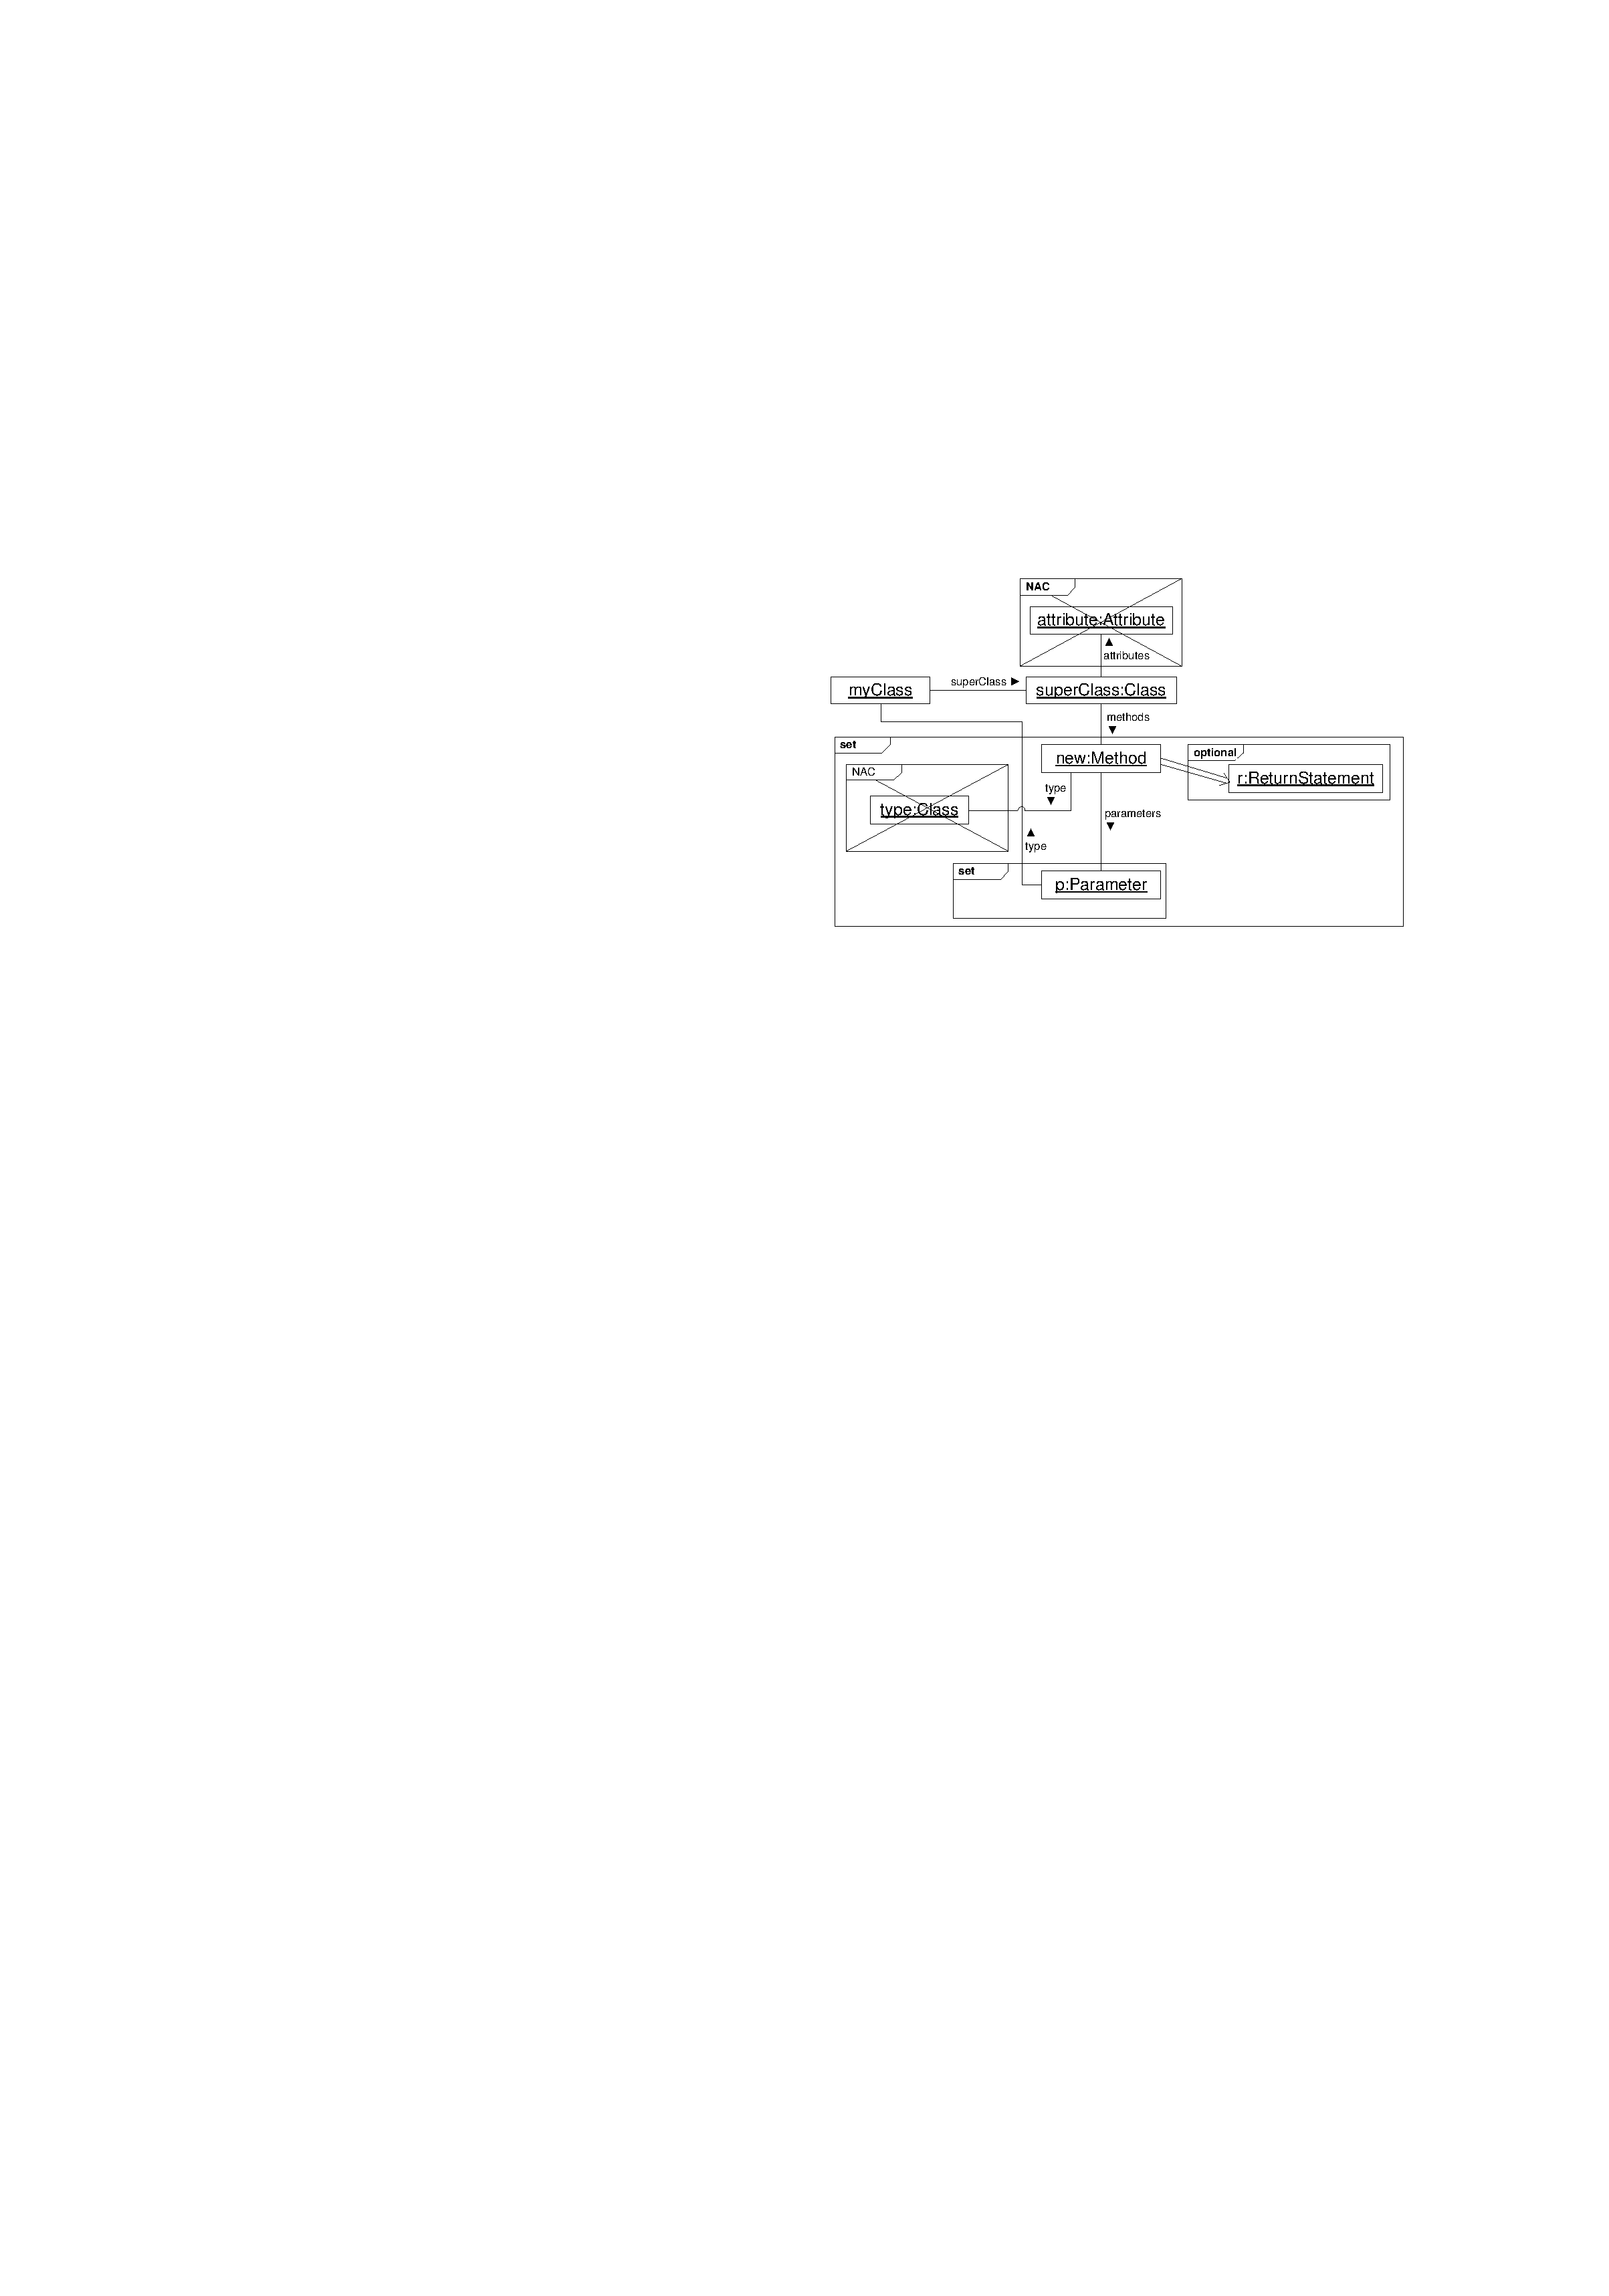
\includegraphics[scale=1.0]{figures/SubPatterns1}
  \caption{Hierarchies of NAC, set, and optional sub patterns}
  \label{fig:subPatternHierarchies}
\end{figure}

\todomcp{How deep may patterns be nested? What is the semantics of alternating binding semantics of sub-patterns, e.g. negative in optional in negative and so on.}
\tododt{I would prefer to allow arbitrarily deep nestings and would suggest to interpret the fragments in the order from outside to inside. Example (see Figure~\ref{fig:subPatternHierarchies}): You match a super class \emph{superClass} of \emph{myClass} and ensure that \emph{superClass} has no attribute. Then you you match all methods \emph{new} (outer set fragment) that have no class as their type (enclosed NAC fragment). Now you match for each of these methods all parameters (enclosed set fragment) that have \emph{myClass} as their type. Furthermore, you try to find a path from the matched \emph{new} method to a return statement (optional fragment).}


